\chapter{Experimental study of the impact of vegetation on the microclimate}
\label{ch:microclimatestudy}
\def\figdir{chapters/ch04_microclimatestudy/figures}

\begin{figure}[h]
	\centering
	\begin{minipage}{0.9\textwidth}
		\textsf{ \footnotesize This chapter is under preparation for publication.}
	\end{minipage}
\end{figure}
\vspace{2em}

\section{Summary}
\lettrine[lines=3,nindent=0em,loversize=0.1]{T}{his} chapter focuses on assessing the impact of vegetation on the microclimate through experimental investigation. The aim of the chapter is to quantify the influence of wind and radiation on the diurnal response of the plant. The influence of vegetation on the microclimate is studied in the wind tunnel using a small \textit{Buxus sempervirens} plant. In the study, the diurnal dynamics of the plant microclimate of a \textit{Buxus sempervirens} is investigated using various high-resolution non-intrusive imaging techniques. The wake flow field is measured using stereoscopic particle image velocimetry (SPIV), the spatiotemporal leaf temperature history is obtained using infrared thermography, and the plant microstructure metrics such as plant porosity, leaf area density (LAD) is obtained through X-ray tomography. The diurnal dynamics of the microclimate of the plant is unveiled using various high-resolution non-intrusive imaging techniques. The wake flow field is measured using stereoscopic particle image velocimetry, the spatiotemporal leaf temperature history is obtained using infrared thermography, and additionally, the plant microstructure metrics such as plant porosity are obtained through X-ray tomography. We find that the wake velocity statistics is not directly linked with the distribution of the porosity but depends mainly on the geometry of the plant foliage which generates the shear flow. The interaction between the shear regions and the upstream boundary layer profile is seen to have a dominant effect on the wake turbulent kinetic energy distribution. Furthermore, the leaf area density distribution has a direct impact on the short-wave radiative heat flux absorption inside the foliage where 50\% of the radiation is calculated to be absorbed in the top 20\% of the foliage. This localized radiation absorption increases the leaf and air temperature substantially, but locally. Furthermore, a comparison of the diurnal variation in the leaf temperature and the net plant transpiration rate enabled us to quantify the diurnal hysteresis resulting from the stomatal response lag. The day of this plant is seen to comprise of four distinct stages of climatic conditions: \textit{no-cooling}, \textit{high-cooling}, \textit{equilibrium}, and \textit{decaying-cooling} stages.

\section{Introduction}

The influence of plants on the microclimate in an urban environment is of growing interest due to the need of mitigating detrimental effects of urbanization and climate change on urban air temperature \citep{Chen2006,Demuzere2014,Dimoudi2003,Matthews2017,Shashua-Bar2009b,Shashua-Bar2000a}. Plants modify the climate by intercepting solar radiation and by extracting heat from the environment through transpiration during photosynthesis \citep{nobel2009physicochemical}. Furthermore, the plant interferes with the airflow, extracting momentum and enhancing turbulent mixing \citep{Finnigan2009, Gromke2014, Sanz2003}. Due to the present growing need to ensure that cities are resilient and can mitigate the rising temperatures, proposed mitigation strategies are to be properly assessed and such assessment requires an adequate characterization of the effects of vegetation. 

Foliage density is known to have an impact on the wind sheltering provided by a plant \citep{Bitog2012b,Bitog2011b,Guan2003,Manickathan2018b}. The aerodynamic properties of vegetation can be expressed simply through porosity and drag coefficient \citep{Grant1998,Guan2003,Manickathan2018b}. The porosity and drag coefficient are known to depend on plant species \citep{Cao2012,Manickathan2018b,Rudnicki2004,Vollsinger2005}, age \citep{Dahle2010} and, for deciduous plants that shed leaves during winter, the parameters have been observed to vary seasonally as well \citep{Dellwik2019,Hwang2011,Maass1995}. It is known that plant porosity can have an impact on turbulent mixing \citep{Bai2012,Hiraoka2008,Manickathan2018b,McClure2017}, which is seen to directly impact the thermal and pollutant dispersion characteristics of air flow \citep{Conan2015,Gromke2008,Gromke2015c,Gromke2008a}. Plants with high foliage density are seen to have a detrimental effect on pollutant dispersion of below-canopy pollutant sources such as automobiles \citep{Nowak2006}. Nevertheless, a high foliage density is also shown to have a beneficial impact on the pedestrian thermal comfort due to increased shading provided by the plant \citep{Hwang2011,Morakinyo2017,Ng2012}. Foliage density is parameterized using the leaf area index (LAI) to describe the net area of leaves and leaf area density (LAD) to describe the foliage distribution within the plant volume. These parameters are typically measured using optical techniques \citep{Cao2012,Grant1998,Guan2003,Liu2018,Manickathan2018b,Phattaralerphong2005} that may compromise on the spatial accuracy and destructive techniques such as defoliation of the plant \citep{Jonckheere2004,ONeal2002}. Solar radiation absorption within the foliage is known to depend primarily on the distribution of the leaf area density \citep{Kichah2012,Manickathan2018a,Park2018}.  A dense plant canopy can result in a significant amount of solar radiation being absorbed resulting in a high leaf-to-air temperature \citep{Hiraoka2005,Leuzinger2007,Manickathan2018a}. Higher plant transpiration is then required to compensate for the high solar radiation absorption \citep{Manickathan2018b}, and this can result in a lower air temperature under the foliage \citep{Wong2003}. Studies have also revealed that plant transpiration rate varies not just due to atmospheric evaporative demand (AED) \citep{Kichah2012,Manickathan2018a,McVicar2012,Tuzet2003} but can also dynamically vary during the day with higher transpiration during morning than in the evening \citep{Huang2017,Tuzet2003}. Therefore, experimental observations allow to determine the diurnal variability in the transpirative cooling performance of vegetation.

Various experimental approaches have been employed to assess the response of plants to environmental conditions ranging from field measurements \citep{Dellwik2019,Grant1998,Hagishima2007,Koizumi2016,Shashua-Bar2009b,Shashua-Bar2000a,Yuan2017}, greenhouse studies \citep{Fatnassi2006,Ganguly2009,Majdoubi2009,Montero2001}, and wind tunnel experiments \citep{Grace1977,Liu2018,Manickathan2018b,Miri2019,Rudnicki2004,Vollsinger2005,Yue2008}. Wind tunnel experiments, which provide the most control over the airflow conditions, typically focus on the aerodynamic characteristics such as drag coefficient, porosity, and sheltering effect of plants and neglect the hygrothermal responses of the plant \citep{Grace1977,Manickathan2018b}. Therefore, the relationship between porosity heterogeneity and hygrothermal conditions of plants has yet not been to be experimentally observed and characterized. Moreover, few studies provide a high-resolution temporal and spatial study of the hygrothermal conditions of the plant which can be used for validating numerical models. Thus, there is a need for high-resolution experimental datasets investigating the links between plant morphology, and aerodynamic conditions including diurnal variations of the hygrothermal conditions such as air temperature, and relative humidity and how all of these affect plant conditions. 

The goal of the study is to experimentally quantifying the influence of plant foliage geometry and environmental conditions such as wind speed and solar radiation on the transpirative cooling performance of a plant (Buxus sempervirens) inside a wind tunnel in a holistic approach. This is achieved by using multiple non-intrusive imaging techniques, thus measuring the plant foliage density with X-ray tomography, the wake flow field using stereoscopic particle image velocimetry (SPIV), the plant leaf temperature with infrared thermography and the hygrothermal conditions inside the foliage using various humidity and temperature sensors. The advantage of X-ray tomography to determine the plant porosity is that it is a non-intrusive approach of determining the plant structure, thus the plant can undergo a series of additional experiments. This approach is inspired from the field of building physics where, for example, the determination of the microstructural morphology of building materials such as asphalt \citep{Lal2016,Lal2017} or materials such as cotton textiles \citep{Parada2017} is used to link the material configuration to its wetting and drying behavior. Thus, the approach allows us to quantify the impact of the plant foliage morphology on the wake flow characteristics, the hygrothermal conditions such as air temperature and relative humidity inside the plant foliage, the solar radiation penetration through the foliage and, finally, on the spatial distribution of the leaf temperature. 

The study aims to answer the questions of how plant cooling varies spatially and temporally under variations of environmental conditions such as wind speed and solar radiation and whether a typical diurnal response of the plant could be defined. Moreover, the experiment provides a high-resolution dataset for future modeling validation studies. Given that this investigation is performed in a wind tunnel, we study the diurnal microclimate of a small plant. A large mature tree will most probably affect its environment in a dissimilar way. For example, the size of the plant, the flexibility of the branches and foliage, etc. can have an influence on the plant aerodynamic responses \citep{DeLangre2008,Manickathan2018b}. 

\section{Materials and methods}

\subsection{Materials}


The measurement campaign was performed for a small Buxus plant (Buxus sempervirens) in a wind tunnel as shown in \cref{fig:plant_setup}. The plant foliage has a dimension $20\times20\times21$ cm$^3$ ($x\times y\times z$, i.e., streamwise, spanwise and vertical) as shown in Fig. \cref{fig:plant_setup}b. The plant was placed in a pot, sealed using putty sealant to ensure water was lost only through leaf transpiration (\cref{fig:plant_setup}c). The water loss due to transpiration was periodically compensated by adding fertilized water ($1$\% (vol.) NPK 7-4-6 Buxus fertilizer). Prior to the experiment, the plant was periodically irrigated and exposed for one week to artificial sunlight with a 12-hour day-night cycle, where day is a fixed-intensity photoperiod. The artificial sunlight was provided using an Osram Ultra-Vitalux $300$ W solar simulator bulb, generating $13.6$ W of UVA and $3.0$ W of UVB. The bulb was placed 60 cm above the plant to provide $100$ W\,m$^{-2}$ plant-canopy incident short-wave radiation. Furthermore, the growth of the plant foliage was periodically maintained to maintain the desired plant geometry as shown in \cref{fig:plant_setup}. The detailed measurement of the plant morphology including geometry, porosity distribution, leaf size distribution, and total leaf area, was obtained using a high-resolution X-ray tomography measurement, as explained below. 

\begin{figure}[t]
	\centering
	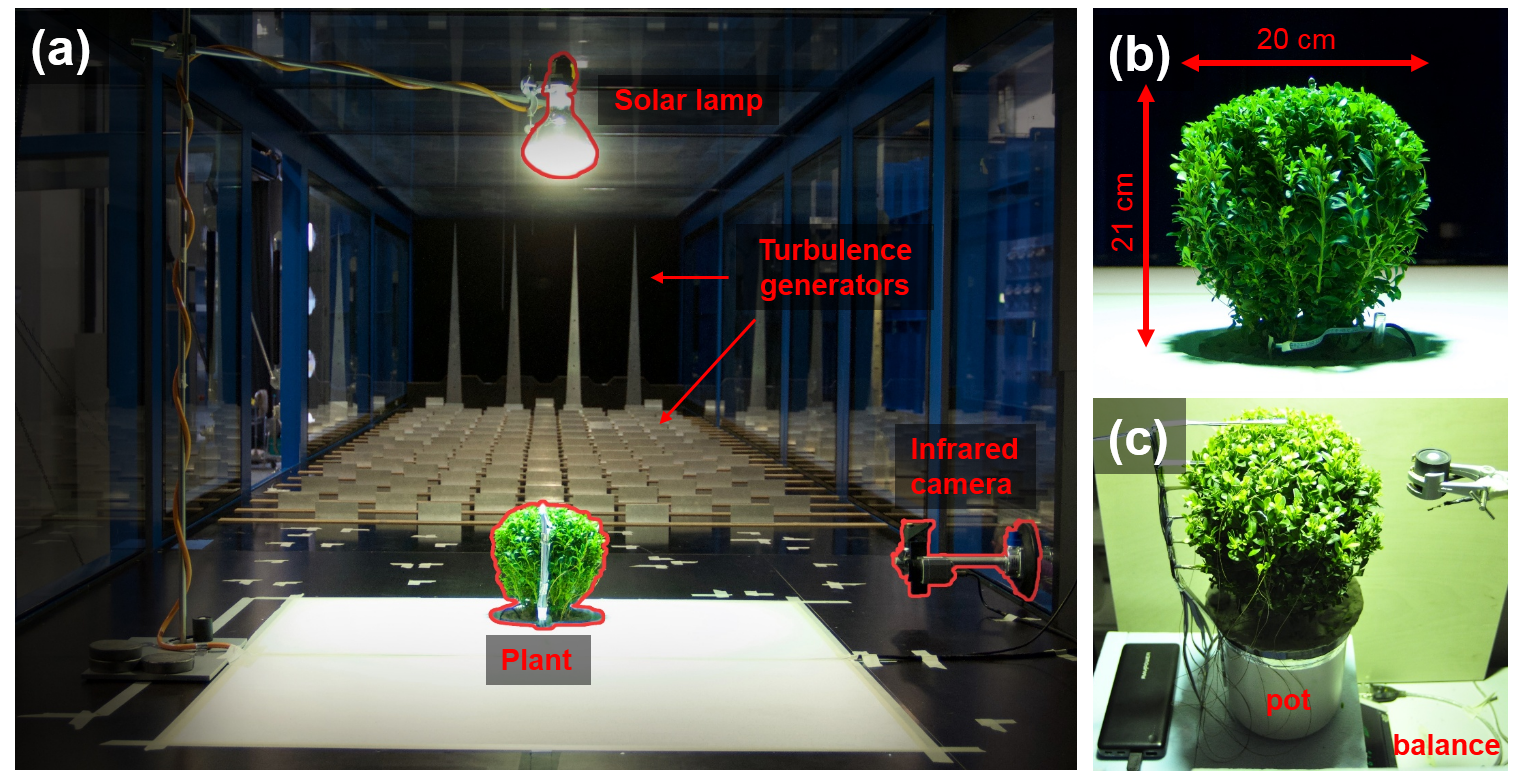
\includegraphics[width=\textwidth]{\figdir/windtunnelsetup_updated_labelled.png}
	\caption{Wind tunnel setting for combined microclimate, SPIV, and infrared thermography measurements: \subfig{a} Photo of plant installed in the tunnel, \subfig{b} A close-up frontal view (windward) of the plant with dimensions, \subfig{c} Photo of pre-experiment plant acclimation setup.}
	\label{fig:plant_setup}
\end{figure}


\subsection{Experimental setup and procedure}

The experimental campaign was divided into three stages: \textit{offline} plant morphology measurement, pre-experimental controlled acclimatization setup, and the wind tunnel experiment. The \textit{offline} measurement aimed to determine the plant morphological properties such as leaf area, porosity and porosity distribution using high-resolution X-ray imaging \cref{subsec:xray}. The aim of the pre-experiment control setup was to acclimatize the plant to the wind tunnel boundary condition of solar radiation diurnal cycle. Furthermore, the sensors required for measuring the air and leaf temperature and air relative humidity within the foliage are mounted at this stage. Finally, the wind tunnel experiment aims at documenting the environmental conditions of the plant subjected to moderate wind. Thus, the flow field downstream of the plant, the hygrothermal microclimate inside the plant, the net transpiration rate and the plant foliage thermal profiles are measured.

\subsection{X-ray imaging}
\label{subsec:xray}

A high-resolution computed tomography (X-ray CT) of the plant is acquired to determine the foliage morphology, the foliage porosity distribution and the net leaf area. The advantage of such an approach is that it is a non-intrusive approach where the same plant can be further investigated \citep{Lal2017,Patera2018}. The measurement is performed at the Diagnostic Imaging Research Unit (DIRU) at the Vetsuisse Faculty, University of Zurich, using a Philips Brilliance CT 16-slice scanner, shown in \cref{fig:xrayimaging}, designed for medical imaging with an acquisition period of $39$ seconds. The CT slices have a resolution of $0.318\times0.318$  mm$^2$ pixel with a slice thickness of $0.4$ mm. The 12-bit image intensity data and the associated data of the measurement are stored in DICOM file format. The resulting X-ray radiation intensity $I$ decay along the path $r$ is dependent on the initial intensity $I_0$ and the spatial distribution of the attenuation coefficient $\mu$ along the path $r$, given by the Beer-Lamberts law:
\begin{equation}
I(r) = {I_0}\exp \left\{ { - \int\limits_0^r {\mu \left( r \right){\mathrm{d}}r} } \right\}
\end{equation}

The plant properties such as net leaf area are obtained from the 3D dataset after image processing, consisting of image enhancement, image segmentation, and classification.

\begin{figure}[t]
	\centering
	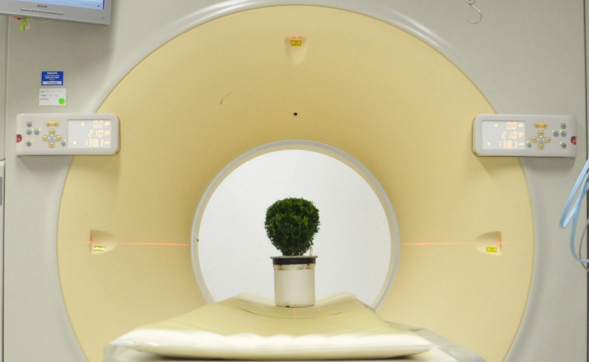
\includegraphics[width=0.7\textwidth]{\figdir/xrayimaging.png}
	\caption{X-ray imaging setup of the plant specimen at Diagnostic Imaging Research Unit (DIRU) at the UZH. The specimen is imaged with Philips Brilliance CT 16-slice scanner, a medical imaging device.}
	\label{fig:xrayimaging}
\end{figure}

\begin{figure}[t]
	\centering
	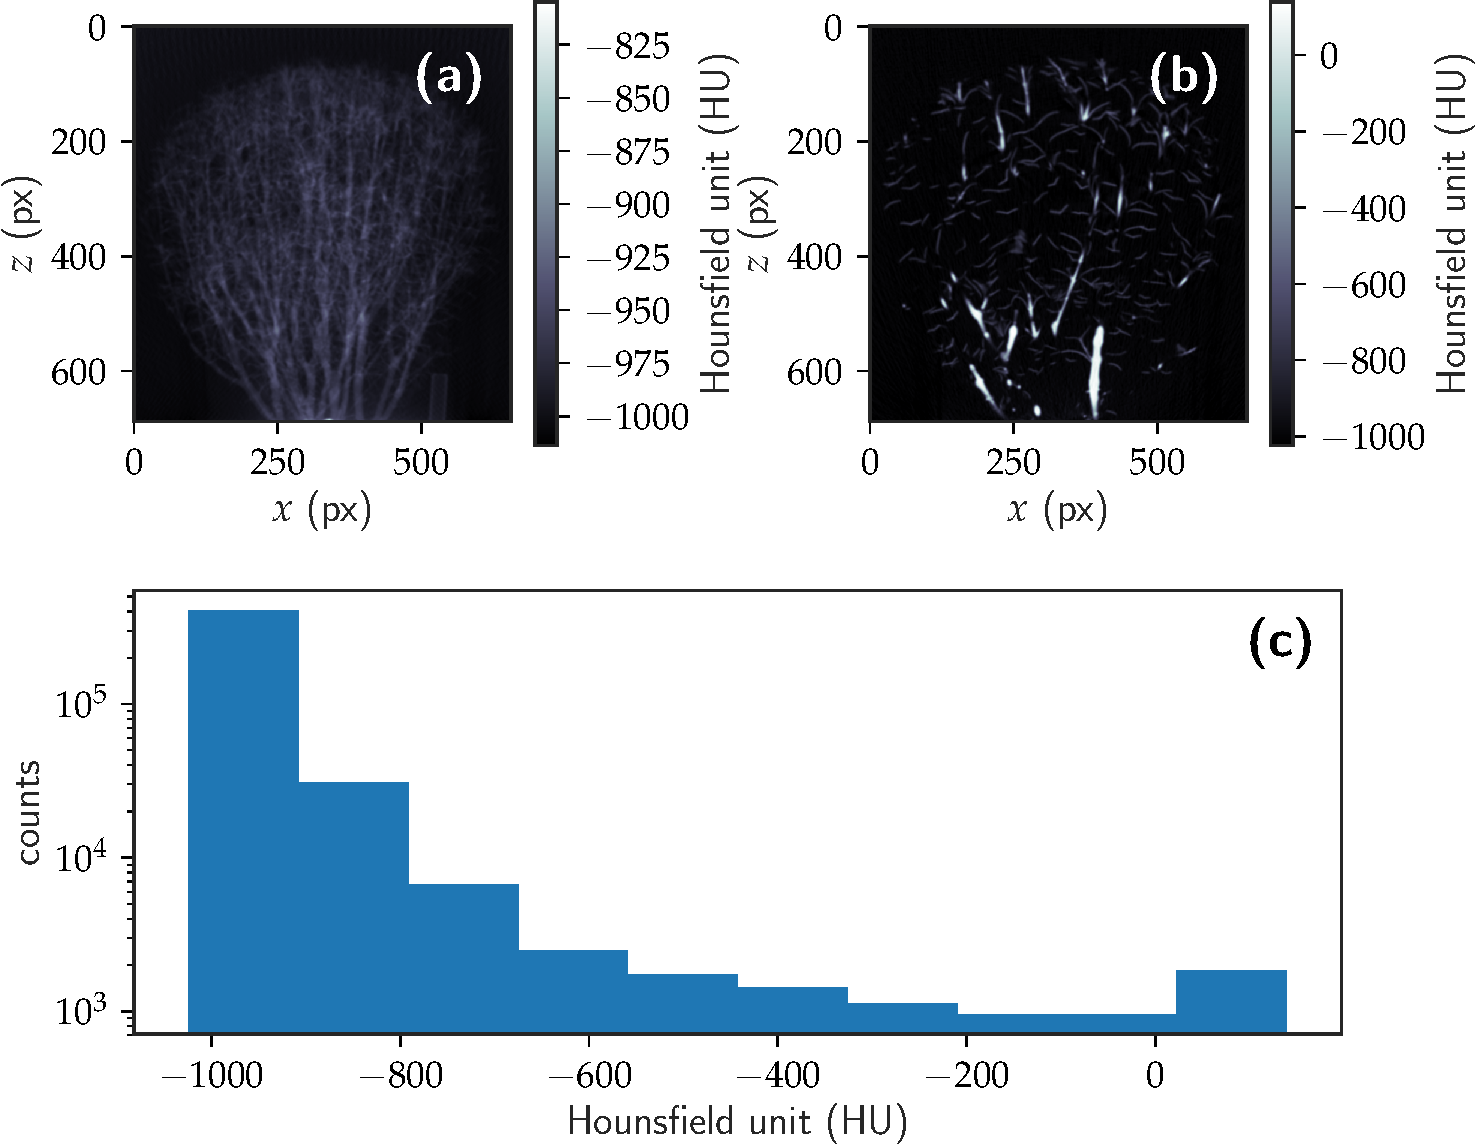
\includegraphics[width=\textwidth]{\figdir/figure_rawimage-crop.pdf}
	\caption{Raw image obtained from x-ray CT-scan: \subfig{a} the side view of CT-Scan, \subfig{b} a single image slice at the middle of the plant, \subfig{c} Histogram of \subfig{b}. The plant attenuation is represented in Hounsfield units (HU) where $-1000$ corresponds to air and $0$ corresponds to pure water. The image slice resolution is $\Delta x = \Delta z=0.318$ mm with a slice thickness of $\Delta y=0.4$ mm.}
	\label{fig:figure_rawimage}
\end{figure}


\subsubsection*{X-ray computed tomography}

The attenuation coefficient indicates the absorption of the biological material to X-ray radiation, indicating the variability in the biological composition of the sample. The reconstructed tomographic data provides the 3D distribution of X-ray attenuation by the sample. The Hounsfield scaling normalizes the X-ray attenuation coefficient μ with that of the air $\mu_{\textit{air}}$ and distilled water $\mu_{\textit{water}}$ at standard atmospheric conditions, where the Hounsfield units of air and water are $HU_{\textit{air}}=-1000$ and $HU_{\textit{water}}=0$, respectively:
\begin{equation}
HU = 1000 \times \frac{{\mu  - {\mu _{\textit{water}}}}}{{{\mu _{\textit{water}}} - {\mu _{\textit{air}}}}}
\end{equation}
HU can be used to extract the biological properties of the plant as the scaling can be a means for fast and simple categorization of biological matter with different water quantity. 

\subsubsection*{Image segmentation}

\cref{fig:figure_rawimage}a shows a side-view of the CT-scan, whereas \cref{fig:figure_rawimage}b shows a single image slice at the middle of the plant. \cref{fig:figure_rawimage}c shows the histogram distribution of the single image slice. A preliminary observation of the images is that air, leaf, and branch show distinct attenuation coefficients for which a manual thresholding of the histogram is performed. Based on the histogram, a simple segmentation assigns air, leaves, and branches. The pixels are assigned as for air ($-1000$ to $900$), leaves ($-900$ to $-700$), branches ($-700$ to $200$), and anything beyond as foreign material. The bounds are determined with the help of $k$-means clustering method assuming a tri-modal distribution (i.e., $k=3$) of the histogram. The histogram of X-ray CT scan (cref{fig:xrayctslice}c) shows that this assumption is not valid, however, this histography-based segmentation serves as a base case for the more advanced segmentation algorithm. \cref{fig:xrayctslice}a shows the original dataset before the classification and \cref{fig:xrayctslice}b shows the histogram-based classification labels. A first observation shows a reasonable classification of the dataset except at boundaries of the branches, due to lower attenuation at the boundaries of the objects.

\begin{figure}[t]
	\centering
	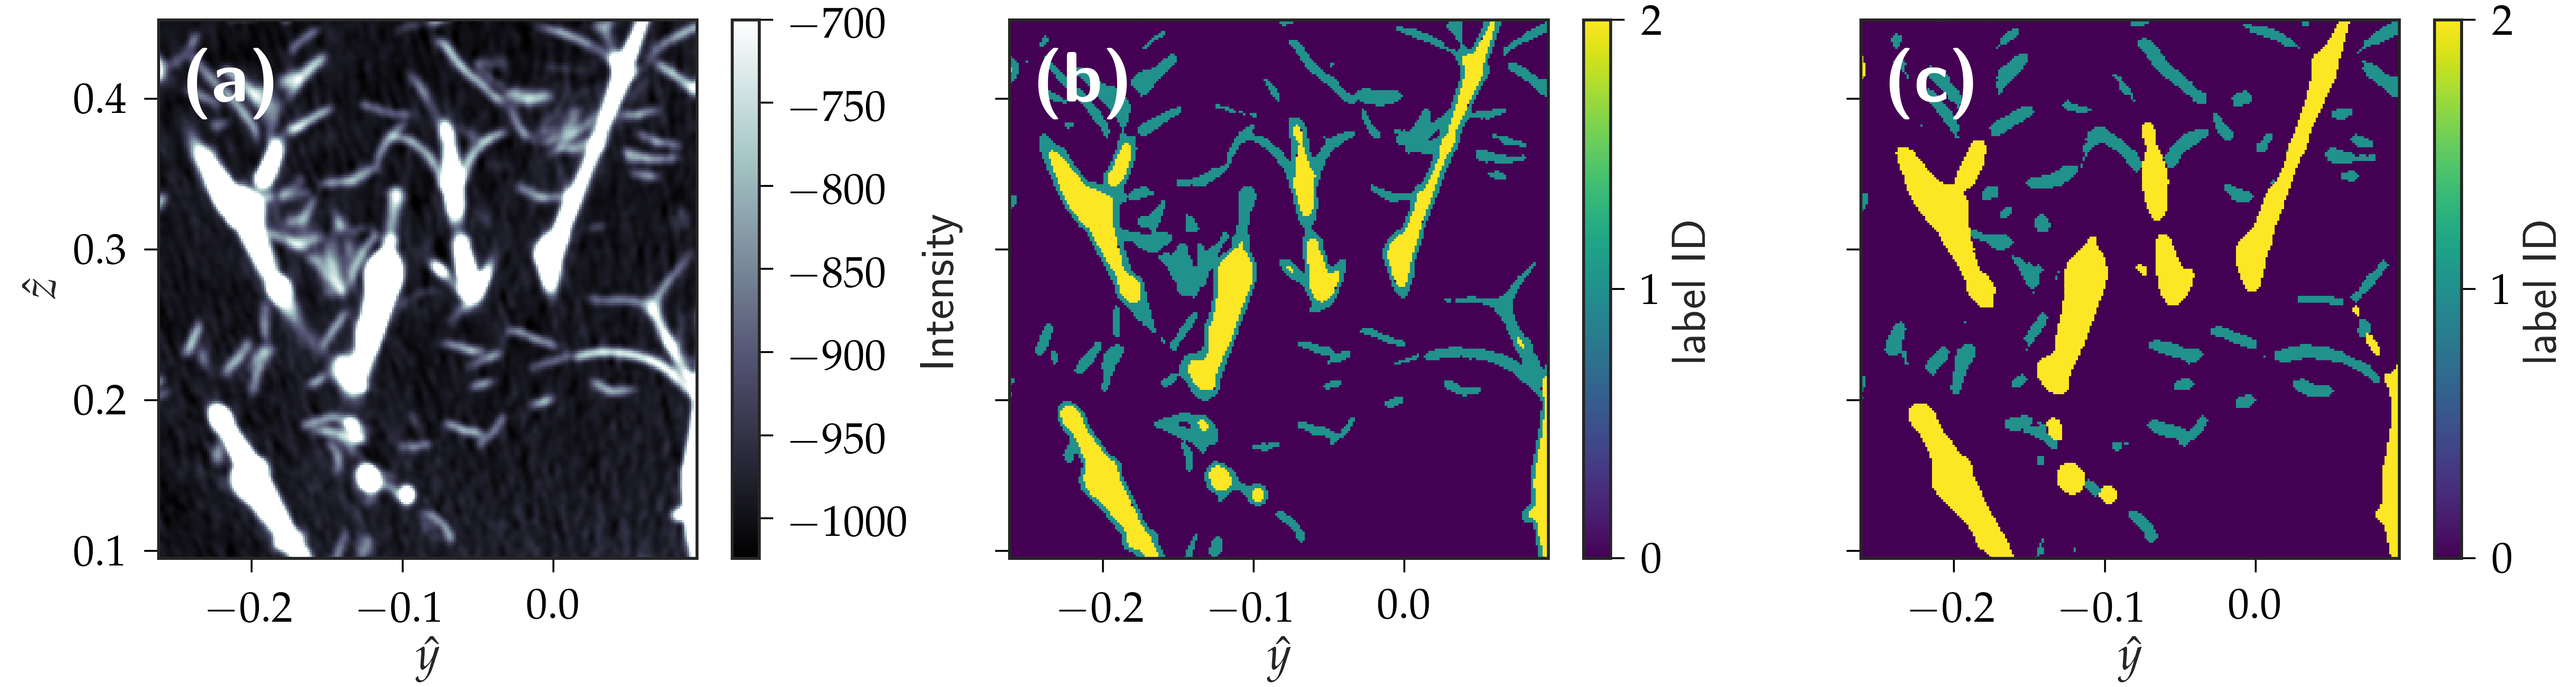
\includegraphics[width=\textwidth]{\figdir/figure_segentation_poster.png}
	\caption{Segmentation of the X-ray CT scan: \subfig{a} slice of original X-ray CT dataset, \subfig{b} segmentation using user-defined histogram threshold and \subfig{c} segmentation using Trainable WEKA Segmentation and additional morphological operation (opening + closing). Only a sub-region of an image slice is shown for clarity. The segmented pixels are labeled as air ($0$, purple), leaf ($1$, blue) and branch ($2$, yellow).}
	\label{fig:xrayctslice}
\end{figure}

Therefore, a more advanced approach, the Trainable Weka Segmentation (TWS) \citep{Arganda-Carreras2017} and additional binary morphological operations are used for classification of the three components of the tree. The TWS segmentation employs an implementation of fast random forest ensemble classification algorithm in the Fiji application \citep{Schindelin2012} using $200$ decision trees with $2$ random features from user selection. A larger selection of edge-enhancement filters is used to reduce the over-estimation of the leaves at the boundary. The training procedure consisted of providing an initially labeled training dataset, trained using the classifier, visually validating the classification, and improving the user-provided labeled training dataset for improved classification. Finally, small remaining leaf pixels at the boundary of the branches were removed using additional morphological operations (\textit{opening} + \textit{closing} \citep{Haralick1987}) using the python library, \texttt{scikit-image} \citep{VanderWalt2014a}. \cref{fig:xrayctslice}c shows the resulting segmentation using the decision tree classification and morphological operation. The figure shows a better classification of the plant elements. From this processed dataset, the plant surface mesh  for branches and leaves can be generated to obtain metrics such as net leaf surface area.


\subsection{Wind tunnel setup}
\label{subsec:windtunnelsetup}

The measurement setup is a holistic measurement approach for simultaneously measuring multiple microclimate parameters. The climate measurements consisted of the measurement of the air relative humidity, air temperature, the net plant transpiration, and the flow velocity. The measurements were performed inside the ETHZ / Empa Atmospheric Boundary Layer (ABL) wind tunnel, a closed circuit G\"ottingen type wind tunnel with a test section cross-section of $1.9\times1.3$ m$^2$ ($W\times H$). The blockage ratio (i.e., the frontal area of the plant to wind tunnel cross-section) of the plant is determined to be $1.7$\% and is, therefore, neglected. \cref{fig:plant_setup}a shows the wind tunnel setup that is employed to ensure minimal disturbances from measurement instruments. During the microclimate measurement, the diurnal variations of the air temperature and relative humidity at different heights were recorded using RH/T (i.e., combined relative humidity and temperature measurement) sensors. In addition, the leaf temperature was measured using infrared thermography. The net transpiration rate from the plant was measured using a mass balance positioned below the wind tunnel floor through an access panel, ensuring that the disturbance of the air flow is affected by the presence of the plant only (Fig. 6b). The airflow leeward of the plant was measured using stereoscopic particle image velocimetry (SPIV). 

The “online” measurement consists of microclimate measurement, where humidity, temperature, and net transpiration rate are measured and airflow measurement, where the wake-flow of the plant is measured. The measured are performed inside the ETHZ / Empa Atmospheric Boundary Layer (ABL) wind tunnel, a closed circuit Göttingen type wind tunnel with a test section cross-section of $1.9\times1.3$ m$^2$ ($W\times H$). The blockage ratio resulted from the plant is $1.7$\%. \cref{fig:plant_setup}a shows the wind tunnel setup that is employed to ensure minimal disturbances from measurement instruments. During the microclimate measurement, the diurnal variation of the air temperature and humidity distribution are recorded using thermocouples and RH/T sensors. Furthermore, the leaf temperatures are measured using an infrared thermography. Additionally, the net transpiration rate from the plant is measured using a mass balance hidden below the wind tunnel through an access panel, ensuring that the disturbance of the air flow is minimized  (\cref{fig:fullsetup}). The coupled measurement setup can be considered as a holistic measurement approach for simultaneously measuring multiple microclimate parameters. Thereafter, the airflow behind the plant is measured using particle image velocimetry (PIV).
	
	\begin{figure}[p]
		\centering
		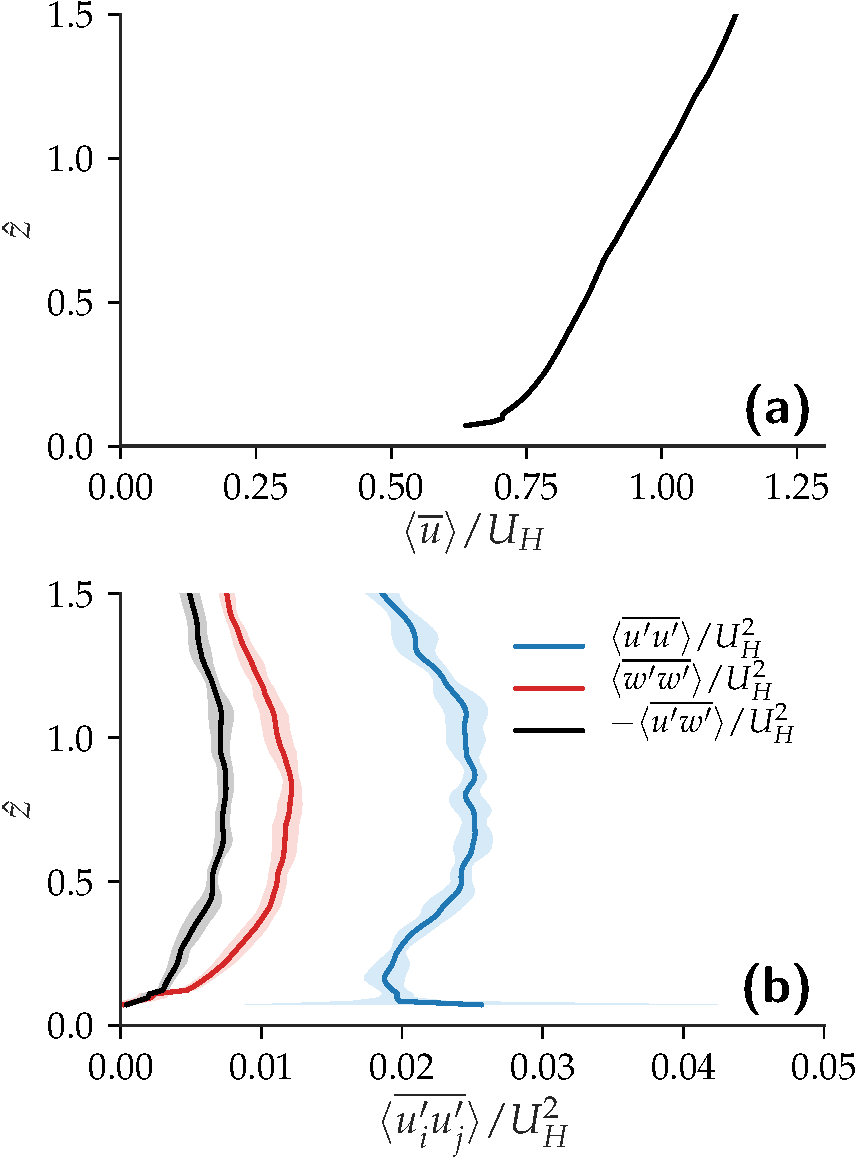
\includegraphics[height=0.7\textheight]{\figdir/figure_incomingvelocityprofile_updated-crop.pdf}
		\caption{Vertical profiles of incoming \subfig{a} normalized mean streamwise velocity $\langle \overline{u} \rangle / U_H$ and \subfig{b} normalized Reynolds stresses $\langle \overline{u'_i u'_j}/U_H^2 \rangle$. The normalized vertical height  $\hat{z}=z/H$. The canopy velocity at $H=210$ mm is $U_H = 0.77$ m\,s$^{-1}$ \citep{Tsalicoglou2018}.}
		\label{fig:incomingvelocityprofile}
	\end{figure}


\subsubsection*{Microclimate boundary conditions}
A parametric study on the steady-state and dynamic response of the plant exposed to four environmental conditions was performed: two wind tunnel set wind speeds, $0$ and $1$ m\,s$^{-2}$, and two plant-canopy incident solar radiation levels, $0$ and $100$ W\,m$^{-1}$. The air temperature and the relative humidity inside the wind tunnel were $21$ $^{\circ}$C and $25$\% RH, where the condition was coarsely regulated by the HVAC system of the wind tunnel facility. 

\cref{fig:incomingvelocityprofile} shows the vertical profiles of the mean upstream streamwise velocity and the Reynolds stresses measured in the empty tunnel at the future position of the plant. At plant canopy height,  $H=210$ mm, the measured mean velocity is $U_H=0.77$ m\,s$^{-1}$  for the wind speed of $U_ref=1$ m\,s$^{-1}$. The wind tunnel flow was modified using turbulence generators, as shown in \cref{fig:plant_setup}a, to generate an appropriate ABL profile typically found in an urban context \citep{Tsalicoglou2018}. \cref{fig:incomingvelocityprofile} shows the mean velocity and variance of velocity profiles that is typical for an ABL, with a turbulent intensity $I=\sqrt{2⁄3\,k}/U_{\textit{ref}}= 12.1$\%. This turbulence intensity thus exposed the plant foliage to air flow characteristics of an urban boundary profile. 


\subsubsection*{SPIV setup}
A stereoscopic particle image velocimetry (SPIV) setup was used to measure the time-averaged 3D wake structure of the plant. To reconstruct the full 3D wake of the plant, the SPIV setup is traversed eight times vertically from $60$ mm from the ground upwards to $270$ mm, at $30$ mm intervals, to produce eight SPIV planes, as depicted in \cref{fig:fullsetup}a. The time-averaged measurements of each plane are then combined to generate a 3D velocity field of the plant wake flow and its associated turbulence statistics. 

The SPIV measurement setup consists of two $2560 \times 2160$ pixel s-CMOS HiSense Zyla camera and a $200$ mJ\,pulse$^{-1}$ (at $15$ Hz) Nd-YAG Litron laser which is traversed together using a high-precision system. The two cameras are placed at $38^{\circ}$ and $0^{\circ}$ normal to the imaging plane. The wind tunnel is seeded with $1$ $\mu$m Di-Ethyl-Hexyl-Sebacat (DEHS) tracer particles and the velocity vectors are calculated using an iterative cross-correlation algorithm of Dantec DynamicStudio with final interrogation area of $32\times32$ px$^2$ and $50$\%  overlap. The field of view (FOV) of a SPIV plane is $438\times559$ mm$^2$ and provides \num{69015} PIV vectors per plane with an in-plane resolution of $2.5$ mm, whereas the plane-to-plane resolution is $30$ mm. To obtain statistically relevant turbulence characteristics, $5000$ images are obtained at $15$ Hz. Furthermore, to ensure low optical inferences during the SPIV measurement, the hygrothermal measurement devices, thermal imaging devices, and the solar lamp had to be removed. The two distinct setups for airflow measurement and hygrothermal measurement are shown in \cref{fig:fullsetup}a and \cref{fig:fullsetup}b, respectively. Furthermore, we assume that the influence of removed devices is minimal for low wind speeds, such as in our case.

	
%	\begin{figure}[t]
	\begin{sidewaysfigure}[p]
		\centering
		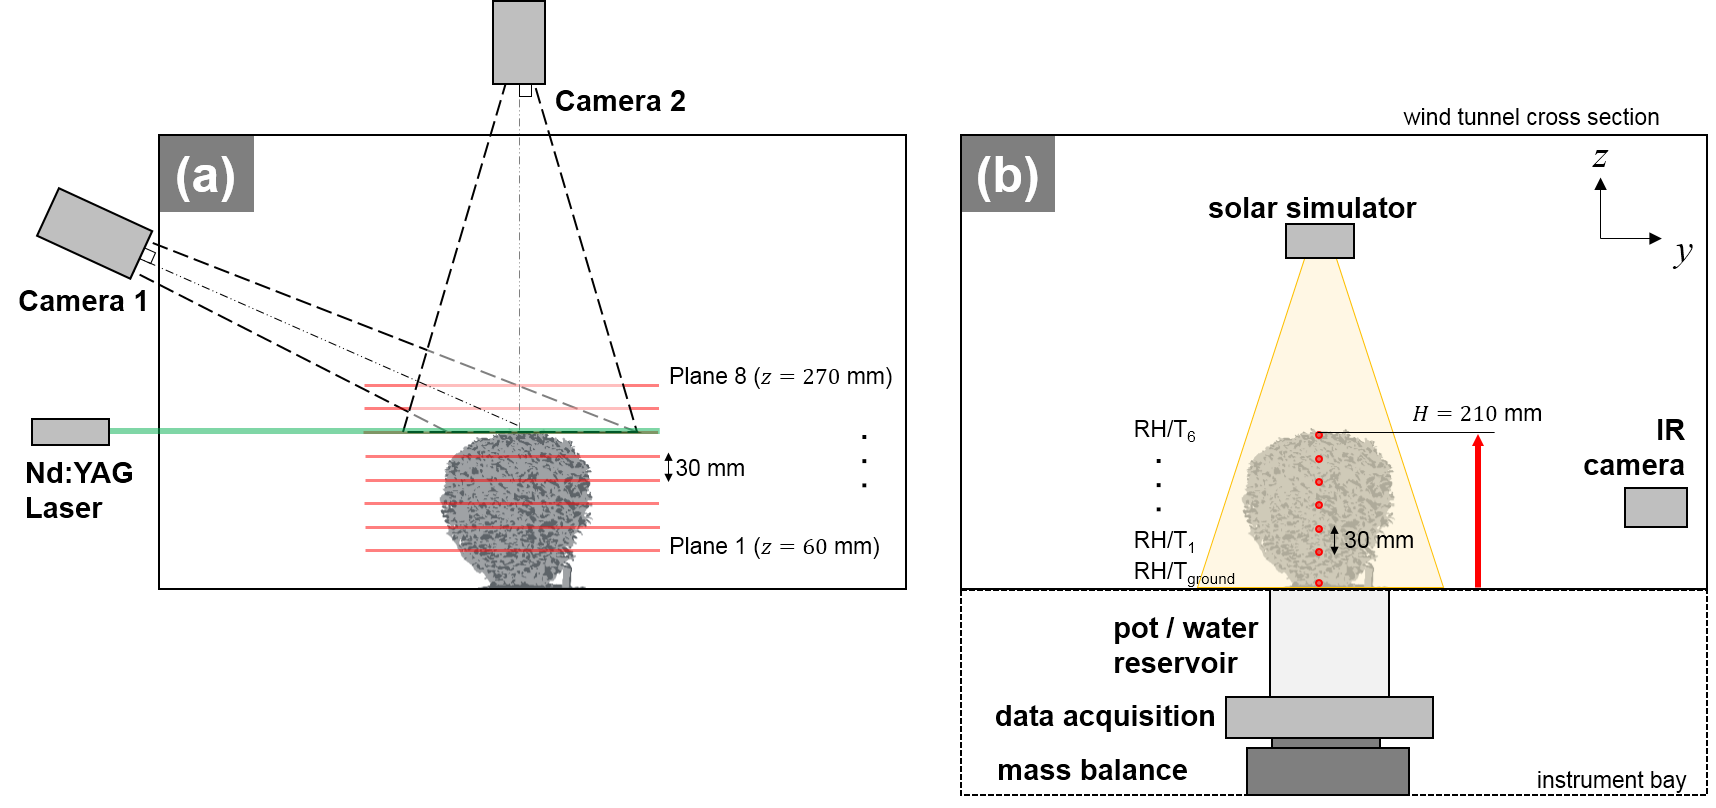
\includegraphics[width=\textwidth]{\figdir/fullsetup.png}
		\caption{Schematic cross section representations of wind tunnel setups used to measure the airflow and hygrothermal microclimate of the plant: \subfig{a} SPIV setup for multi-plane time-averaged measured velocity consisting of eight horizontal planes, $z=[60,90,120,150,180,210,240,270]$ mm, \subfig{b} microclimate measurement setup consisting of IR camera and SHT sensors inside the wind tunnel, mass balance and other data acquisition system below the wind tunnel through an access panel. We note the presence of the solar simulator in the second setup. The two distinct setups are required to attain non-interfered optical measurements of the SPIV.}
		\label{fig:fullsetup}
	\end{sidewaysfigure}
	%	\end{figure}
	
\subsubsection*{Microclimate and net transpiration rate measurement}
The hygrothermal microclimate conditions within the foliage at various wind and radiation conditions are investigated separately from the flow field measurements, as clarified in \cref{fig:fullsetup}. \cref{fig:fullsetup}b shows the setup used to measure the hygrothermal microclimate of the plant. The solar simulator is placed above the plant providing $100$ W\,m$^{-2}$ of incident short-wave radiation at the plant canopy ($H=210$ mm). The solar simulator is controlled using a time switch that provides 12-hour periods of $0$ and $100$ W\,m$^{-2}$ radiation in alternance, imposing a simplified diurnal solar cycle. A fixed radiation intensity was imposed to obtain the steady-state response on the plant. In future, a time-dependent intensity profile such as sine profile can be investigated. The net plant transpiration is measured using a Mettler PM6100 mass balance placed below the wind tunnel floor in the instrument bay along with the plant pot and water reservoir and the data acquisition system, to minimize their inferences on the flow field. The mass balance has a maximum capacity of $6.1$ kg with an accuracy of ($\pm 0.1$ g). Simultaneously, the vertical relative humidity and temperature profiles inside the plant are measured using Sensirion SHT35 sensors, as indicated in \cref{fig:fullsetup}b. Seven SHT sensors are placed as follows: five sensors are directly inside the foliage with a vertical offset of $30$ mm starting below the plant canopy (i.e., $z=[60,90,120,150,180]$ mm), one sensor is at plant canopy (i.e., $z=210$ mm), and one sensor is below the plant foliage near the ground (i.e. $z=0$ mm), to measure the shaded conditions. An eighth sensor is placed directly downstream of the plant at the height of plant canopy (i.e., $z=210$ mm). The eight SHT sensors have an accuracy of $\pm1.5$\% RH (between $0$ and $80$\% RH) and $\pm0.1$ $^{\circ}$C (between $20$ and $60$ $^{\circ}$C). All the sensors for the plant are connected and powered by the wireless data acquisition system directly below the plant pot, such system is necessary to not hinder the mass balance measurement of water loss due to transpiration. The wireless data acquisition system consists of an Arduino Micro and a $\num{20100}$ mAh powerbank providing the necessary power for a multi-day measurement period. The Arduino Micro serves not only as an analog-to-digital signal converter but also as a telemetry device for sending the acquired data to the data logger away from the measurement setup. The data is acquired at a 30-second interval. 


\subsubsection*{Infrared imaging}
Infrared (IR) thermography is performed to obtain a high-resolution spatial and temporal data of the foliage temperature when exposed to varying environmental conditions. The feasibility of employing infrared thermography to obtain leaf temperature variability has been demonstrated in the past \citep{Jones1999,Merlot2002}. IR imaging system is employed to measure the outer plant foliage temperature simultaneously with the hygrothermal and net transpiration rate measured for two different wind conditions throughout the diurnal radiation cycle. The IR imaging system consists of the Optris PI 640 IR camera with a $640\times480$ px$^2$ sensor, a spectral response between $7.5$ and $13$ $\mu$m and is set to measure $-20$ to $100$ $^{\circ}$C  with an accuracy of $\pm2$ $^{\circ}$C  \citep{Allegrini2018,Tsalicoglou2018}. A $33^{\circ}$ lens is used providing an effective FOV of $223\times211$ mm$^2$. The IR measurement is performed at a frequency of 1 frame\,minute$^{-1}$ throughout the diurnal cycle. A PT100 (platinum resistance thermometer) sensor is placed in FOV of the IR image for calibration \citep{Allegrini2018}.


\section{Results and discussion}

%Firstly, the plant traits such as foliage geometry, porosity distribution, and leaf area are derived from the x-ray tomography \cref{subsec:xraytomo}. We show that such properties can be derived with the benefit of being a non-destructive and furthermore provides spatial resolution, which is not possible in other state-of-art techniques. Thereafter, the wake flow field resulting from the foliage heterogeneity is investigated using stereoscopic particle image velocimetry (Stereo-PIV), detailed in \cref{subsec:stereopiv}. The necessity of such a technique is verified from the 3D nature of the flow field. The influence of the heterogeneous porosity distribution and the 3D wake flow field on the plant behavior is investigated at two timescales: firstly, the diurnal response of the plant identifying daytime and nighttime averages (\cref{subsec:diurnal}); and secondly, identifying the dynamic responses of the plant resulted from the plant hysteresis that is seldom modeled in microclimate models with vegetation (\cref{subsec:dynamic}). 


\subsection{X-ray tomography: A non-destructive approach to obtain plant traits}

\subsubsection*{Porosity distribution} 

To calculate the porosity distribution of plant, a valid representative element volume size has to be chosen to represent the plant foliage as a porous media. \cref{fig:porositydistribution}a shows the average porosity for voxel size ranging from $5$ to $100$ px$^3$. The average plant porosity is converged once a sufficiently large REV prescribed. However, a too large REV can reduce the porosity distribution resolution. Therefore, in our case, a REV size of $30$ px$^3$ is seen to be optimal provide sufficient accuracy of average porosity and sufficient spatial resolution. The resulting average plant porosity is $\phi= 0.881$. 

	\begin{figure}[p]
		\centering
		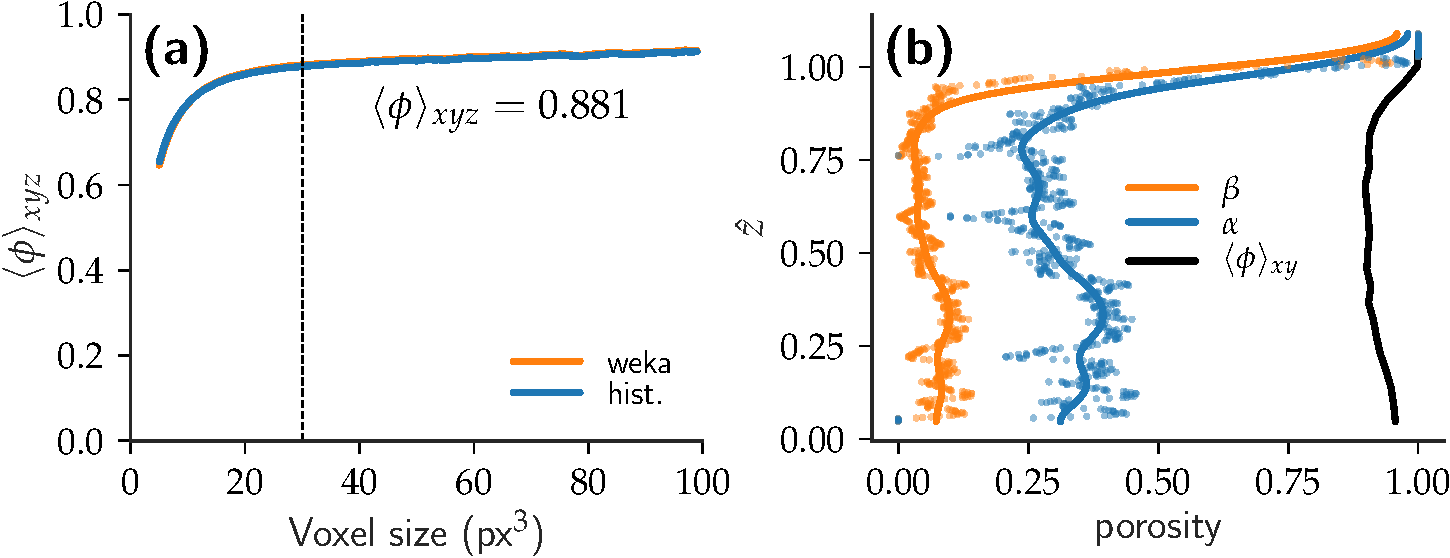
\includegraphics[width=\textwidth]{\figdir/porosity_verticaldistribution-crop.pdf}
		\caption{Determining the representative elementary volume for calculating porosity distribution: \subfig{a} Convergence of average plant porosity $\langle \phi \rangle_{xyz}$ with respect to voxel size (px$^3$) and \subfig{b} Various vertical porosity distribution: optical $\beta$, aerodynamic $\alpha$ and true porosity $\langle \phi \rangle_{xy}$.}
		\label{fig:porositydistribution}
	\end{figure}

	\begin{figure}[p]
		\centering
		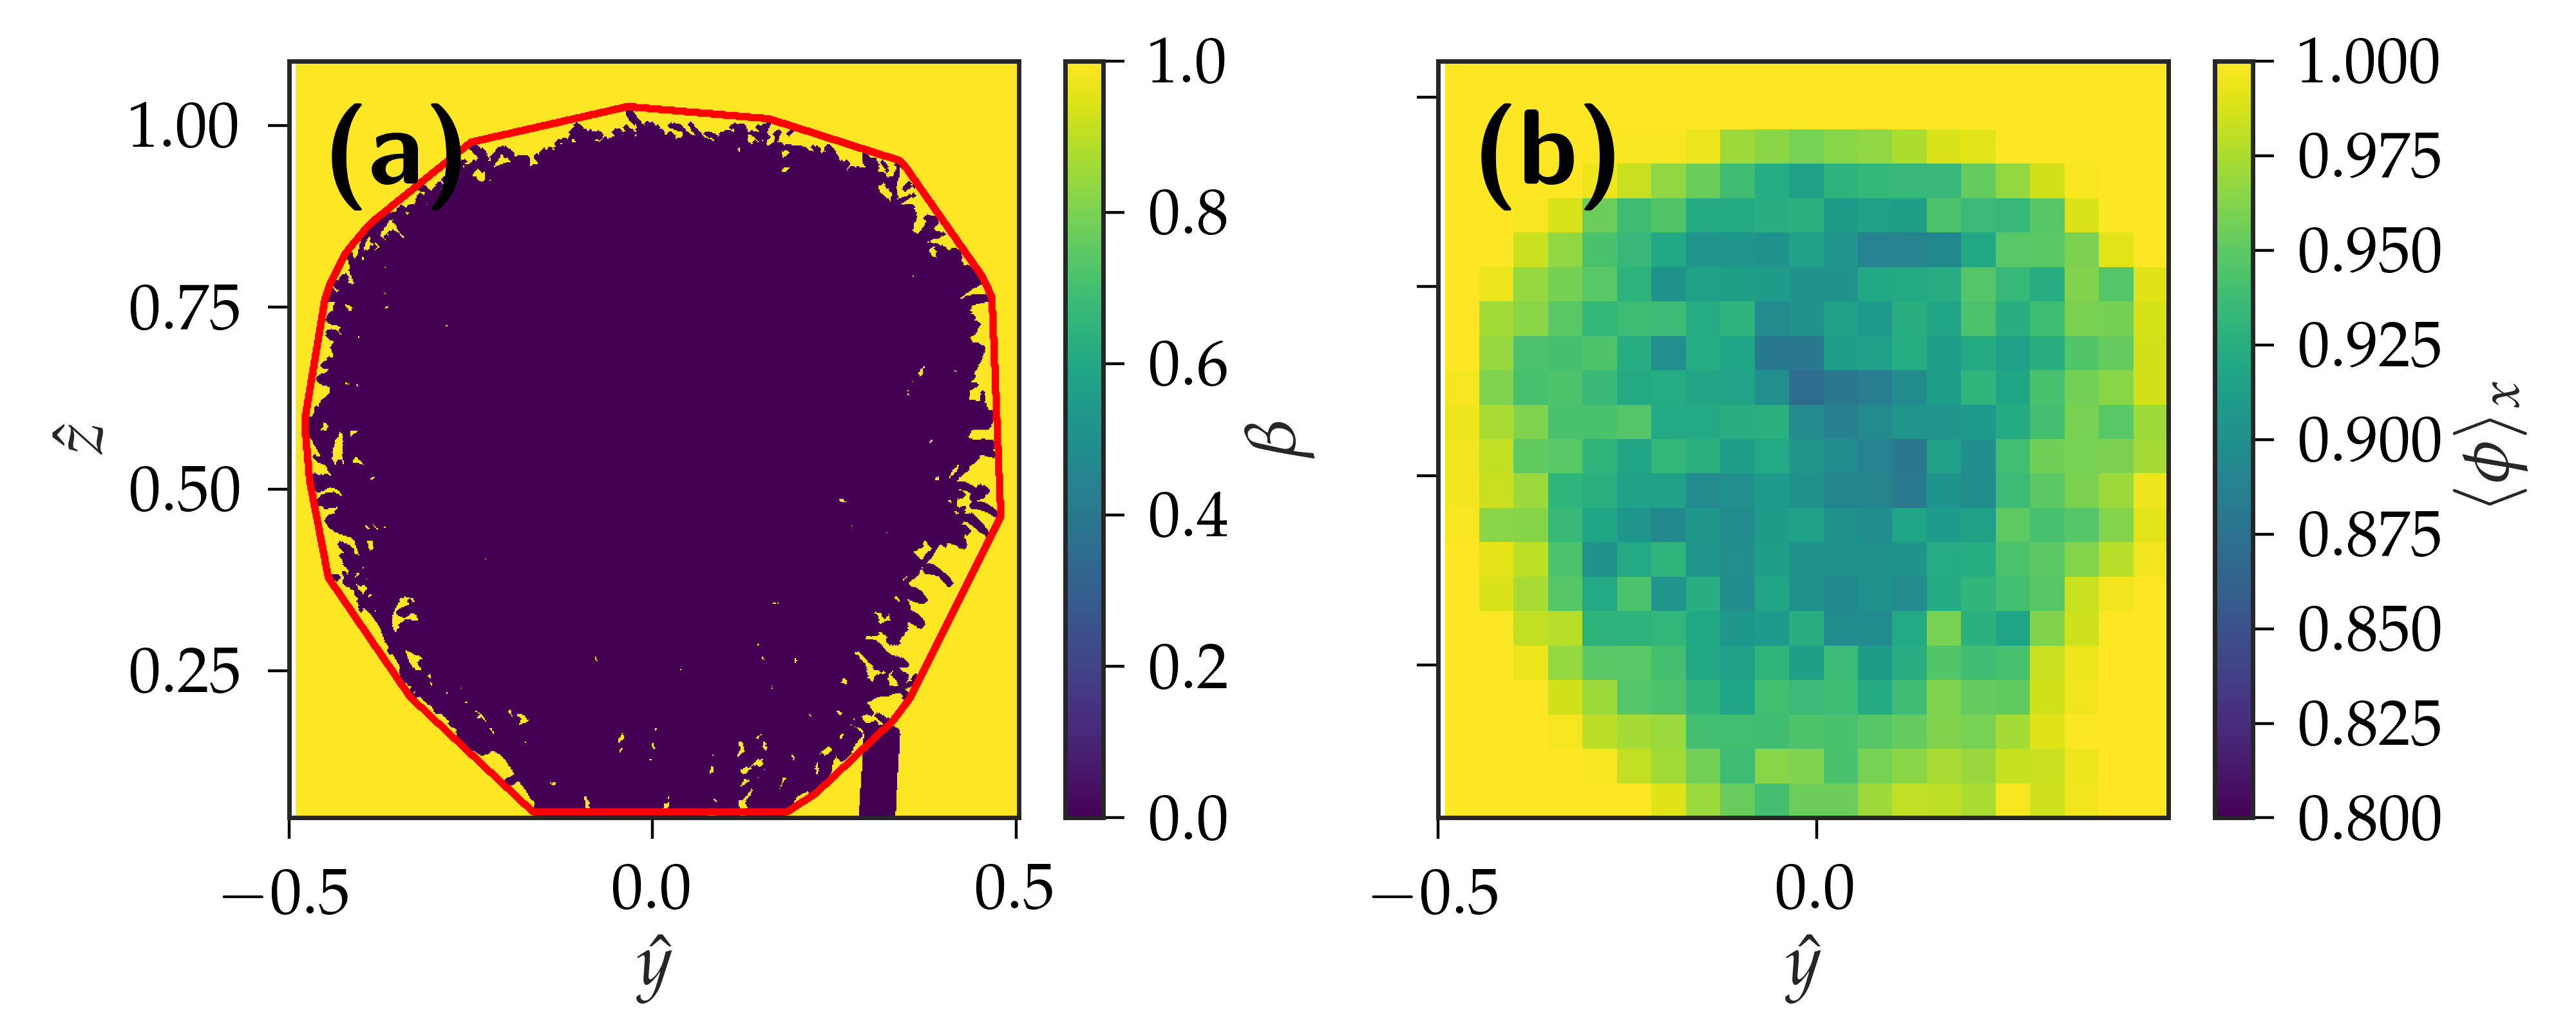
\includegraphics[width=\textwidth]{\figdir/optical_aerodynamic_true_porosity_distribution_type2.png}
		\caption{Porosity distributions of the plant: \subfig{a} The optical porosity $\beta$ with plant element and airspace indexed as $0$ and $1$, respectively and \subfig{b} streamwise-averaged plant porosity $\langle \phi \rangle_x$. }
		\label{fig:porosities}
	\end{figure}

\cref{fig:porositydistribution}b shows the vertical distribution of various porosities. In conjunction with the measured plant porosity (black line), the optical of the plant (with respect to the incident airflow in wind tunnel) is investigated. The optical and the aerodynamic porosity derived from this, are a typical measure used in the wind tunnel studies to estimate the aerodynamic contribution of the plant porosity \citep{Grant1998, Guan2003, Manickathan2018b}. The optical porosity $\beta$ and the aerodynamic porosity $\alpha$ are related as follows:
\begin{equation}
\alpha = \beta^{0.4}
\end{equation}
and in an empirical relationship. The optical porosity is obtained from a 2D optical image of the tree incident to the flow (\cref{fig:porositydistribution}a) and is defined as the ratio of empty pixels (without plant elements) to the total number of pixels within the silhouette of the plant, shown in  \cref{fig:porosities}a. A convex hull is used to define the silhouette of the plant. Furthermore, the streamwise-averaged plant porosity is investigated to quantify the amount of plant elements that will block the flow field at a given location, as shown in \cref{fig:porositydistribution}b. It indicates clearly that the highest blockage is found at the higher-middle region on the plant. Such location of high plant foliage density could indicate high solar radiative absorptions and a resulting high transpiration rate. A measure of the climatic conditions such as air temperature and relative humidity could indicate this hypothesis and show the regions of high transpiration. The plant foliage density is seen to reduce towards to the edges gradually and at these regions, a lower blockage might be present with a higher bleed flow. Furthermore, at locations with the higher bleed flow can provide internal ventilation, increasing the convective dominated processes such as sensible and latex heat flux \citep{Manickathan2018a}. Investigating the plant wake flow can, therefore, provide a better indication of the impact of the heterogeneity in the porosity distribution.

The horizontal-averaged ($x-y$ plane) porosity distribution is shown and compared in \cref{fig:porosities}b. Comparing optical, aerodynamic and true porosity, we see that the true porosity of the plant is substantially higher than the optical and the aerodynamic porosity, especially away from the plant canopy. Therefore, the flow field study can additionally indicate the efficacy of employing aerodynamic porosity vs. true plant porosity on quantifying the sheltering effect of the plant. 

\subsubsection*{Plant surface mesh and total leaf area}

\begin{figure}[t]
	\centering
	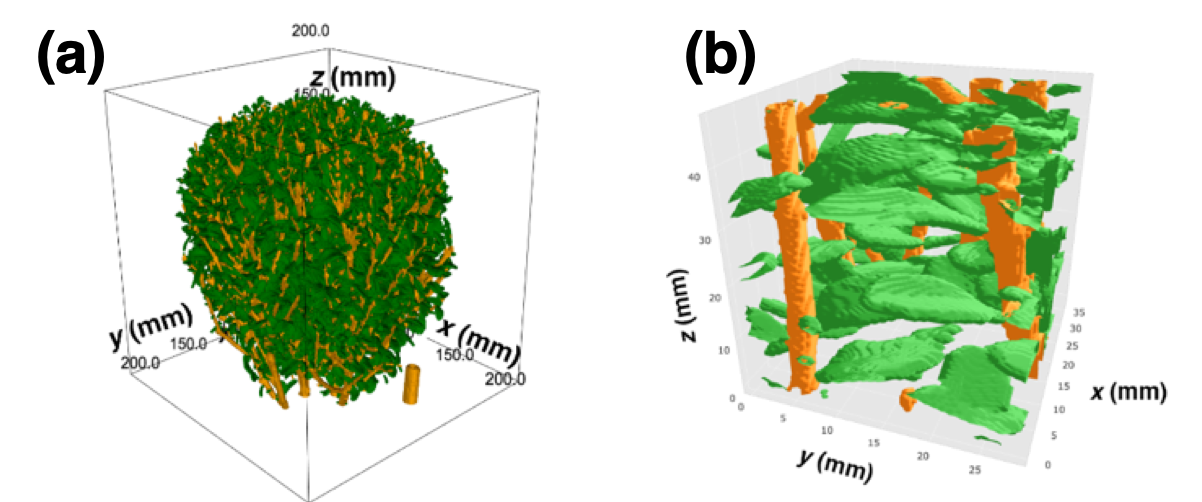
\includegraphics[width=\textwidth]{\figdir/plantmesh.png}
	\caption{Surface geometry of the plant, where leaves (green) and branches (orange) are differentiated: \subfig{a} complete plant surface, \subfig{b} sub-volume inside the plant foliage.}
	\label{fig:plantmesh}
\end{figure}

In addition to the porosity distribution of the plant, the total leaf area and the resulting leaf area index and leaf area density are important parameters for understanding and modeling the influence of vegetation \citep{Manickathan2018a}. The benefit of X-ray tomography is further evident as this parameter can not only be obtained using is a non-destructive but is also an accurate approach to estimate the spatial variability. Typically, the leaf area index (or density) is measured simply from optical measurements or by defoliating the entire plant \citep{Guan2003,Jonckheere2004,Manickathan2018b}. In our study, these plant traits are directly obtained from the x-ray tomography. To achieve this, the surface of the plant elements is generated from the volumetric data of the plant X-ray CT. \cref{fig:plantmesh}a shows the leaf and branch surface colored as green and orange, respectively. \cref{fig:plantmesh}b shows an internal sub-volume of the plant for clarity, and it is observable that the classification has been successful. The surface geometry is generated using a marching-cube algorithm implemented in \texttt{scikit-image} \citep{VanderWalt2014a}.

The total leaf surface area is simply the integral of the surface measure and is calculated to be $A_l=0.75$ m$^2$. A more general measure that is used to qualitatively and quantitatively indicate the amount of leaves is the leaf area index (LAI). The leaf area is defined as the ratio of one-sided leaf area the plant ground cover area:
\begin{equation}
\textit{LAI} = \frac{A_{\textit{l,one-sided}}}{A_g}
\end{equation}
The one-sided leaf area is simply half the total measured leaf area, and the plant ground cover area is obtained directly from the X-ray CT dataset. The plant ground cover was also determined to be $A_g=0.031$ m$^2$, and a resulting leaf area index of $LAI=12.14$ m$^2$\,m$^{-2}$ is measured. Thus, an average leaf area density of $LAD=57.79$ m$^2$\,m$^{-3}$ for a plant height of $H=210$ mm.

\subsection{Stereoscopic particle image velocimetry: 3D wake flow characterization }
\label{subsec:stereopiv}

To study the influence of the plant morphology, measured through X-ray tomography in \cref{subsec:xraytomo}, on the flow field, a stereoscopic particle image velocimetry (Stereo-PIV) approach is employed. Furthermore, to study the resulting 3D wake flow field of the plant and the impact of heterogeneous porosity distribution, the stereo-PIV system measures multiple horizontal planes to capture the full time-averaged plant wake. The setup of the PIV system is detailed in \cref{subsec:windtunnelsetup}, measuring 8 horizontal planes behind the plant at vertical heights of $h =$ $[60$, $90$, $120$, $150$, $180$, $210$, $240$, $270]$ mm.

\subsubsection*{Normalized mean velocity magnitude}
	
\begin{sidewaysfigure}[p]
	\centering
	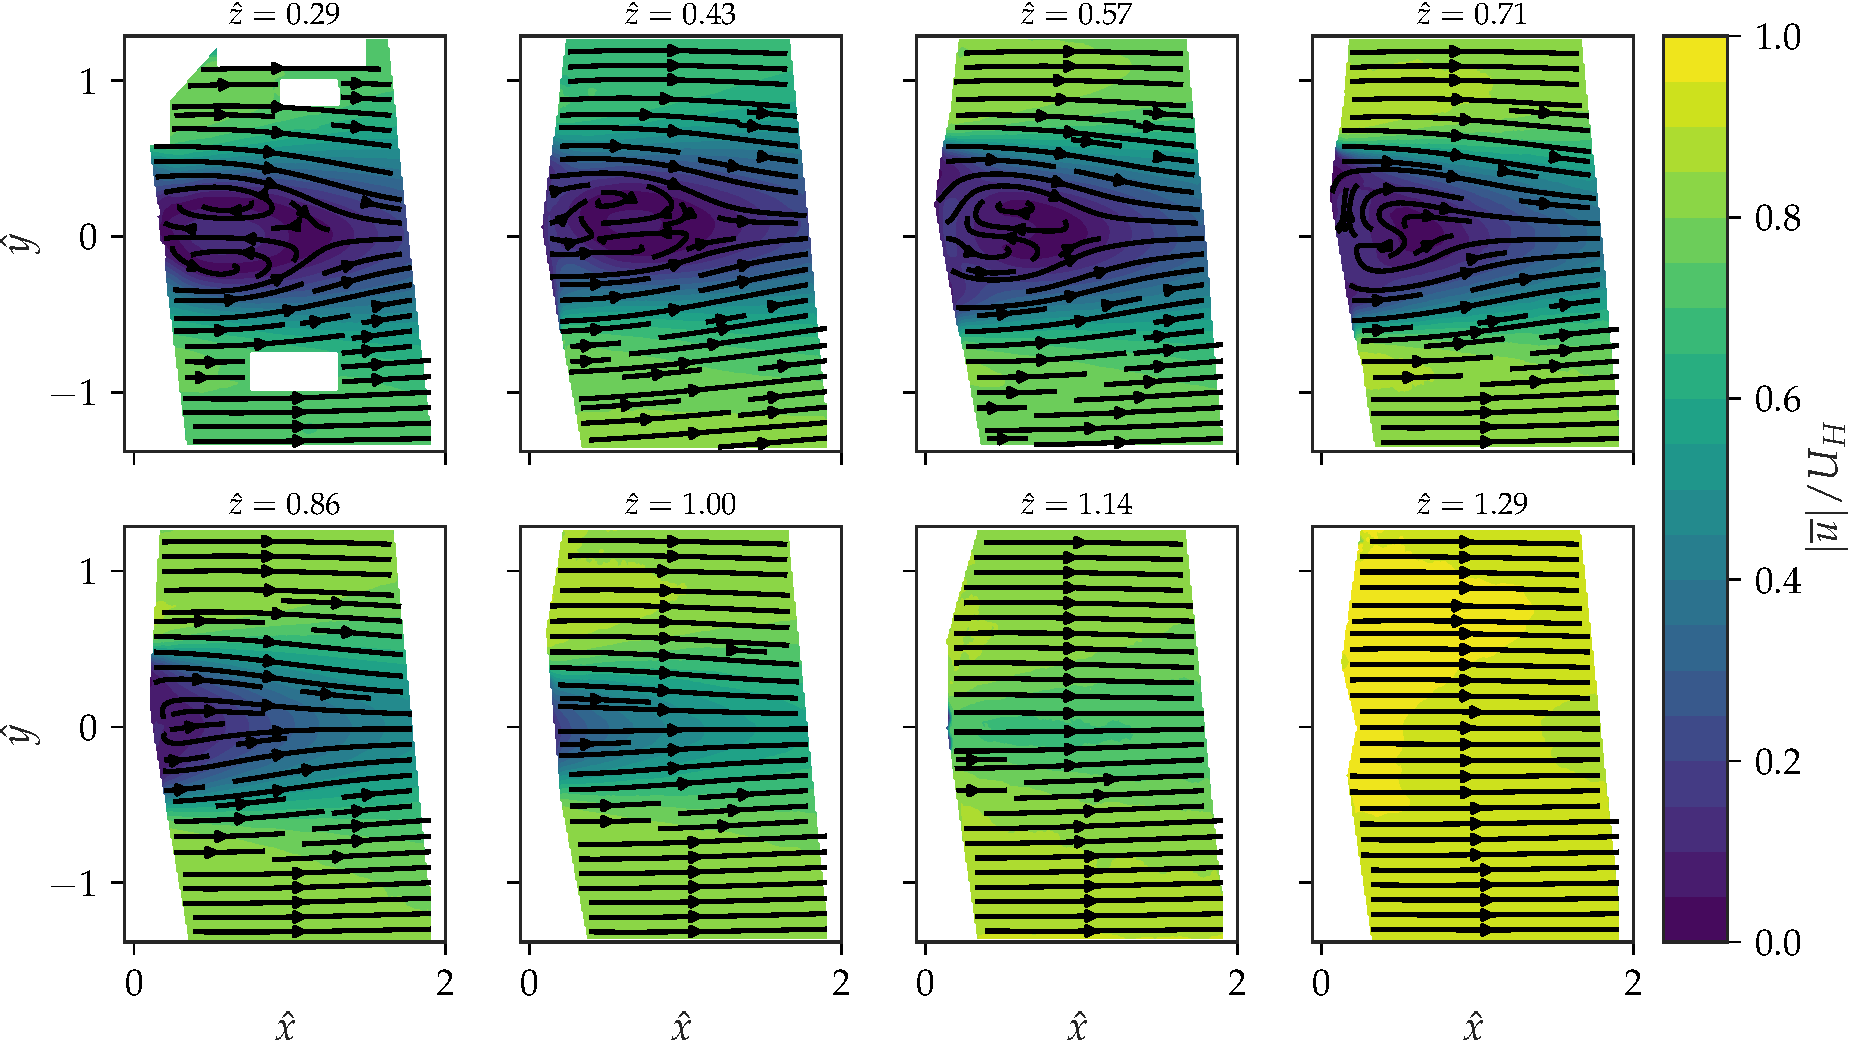
\includegraphics[width=\textwidth]{\figdir/hAll_velocitymagnitude-crop.pdf}
	\caption{Normalized mean velocity magnitude $\tavg{\mvec{u}}/U_H$ at 8 horizontal planes, $\hat{z}=$ [$0.29$,\,$0.43$,\,$0.57$, $0.71$, $0.86$, $1.0$, $1.14$, $1.29]$.}
	\label{fig:meanflow}
\end{sidewaysfigure}

The measurement planes up to a height of $210$ mm are directly in the wake, and the last two heights measure the above-canopy zone. The goal of these exhaustive measurements is to quantify the spatial variability of the plant wake and the 3D nature of the flow generated from the isolated plant. \cref{fig:meanflow} shows the normalized mean velocity magnitude $|\tavg{\mvec{u}}|/U_H$. The coordinate system is normalized with the tree height of $H=210$ mm, where $\hat{x}_i = x_i / H$ for $x_i =\{x,y,z\}$. The mean velocity distribution shows a prevailing recirculation flow for $\hat{x} \le 0.71$, which indicates a wake flow with low bleed-flow. However, further above the tree, the wake flow structure is indicative of bleed-flow showing non-circulating streamlines. Once we investigate the vertical porosity distributions, \cref{fig:porosities}b, we realize that above $\hat{z}>0.71$, the porosity distribution quickly increases to $\phi=1$, correlating the observed bleed-flow from PIV measurement. To further study the impact of such flow configuration on the climate, the influence of the flow conditions on the microclimate inside the plant must be investigated (\cref{subsec:diurnal}). 


\subsubsection*{Turbulent kinetic energy budget}
		
	\begin{sidewaysfigure}[p]
		\centering
		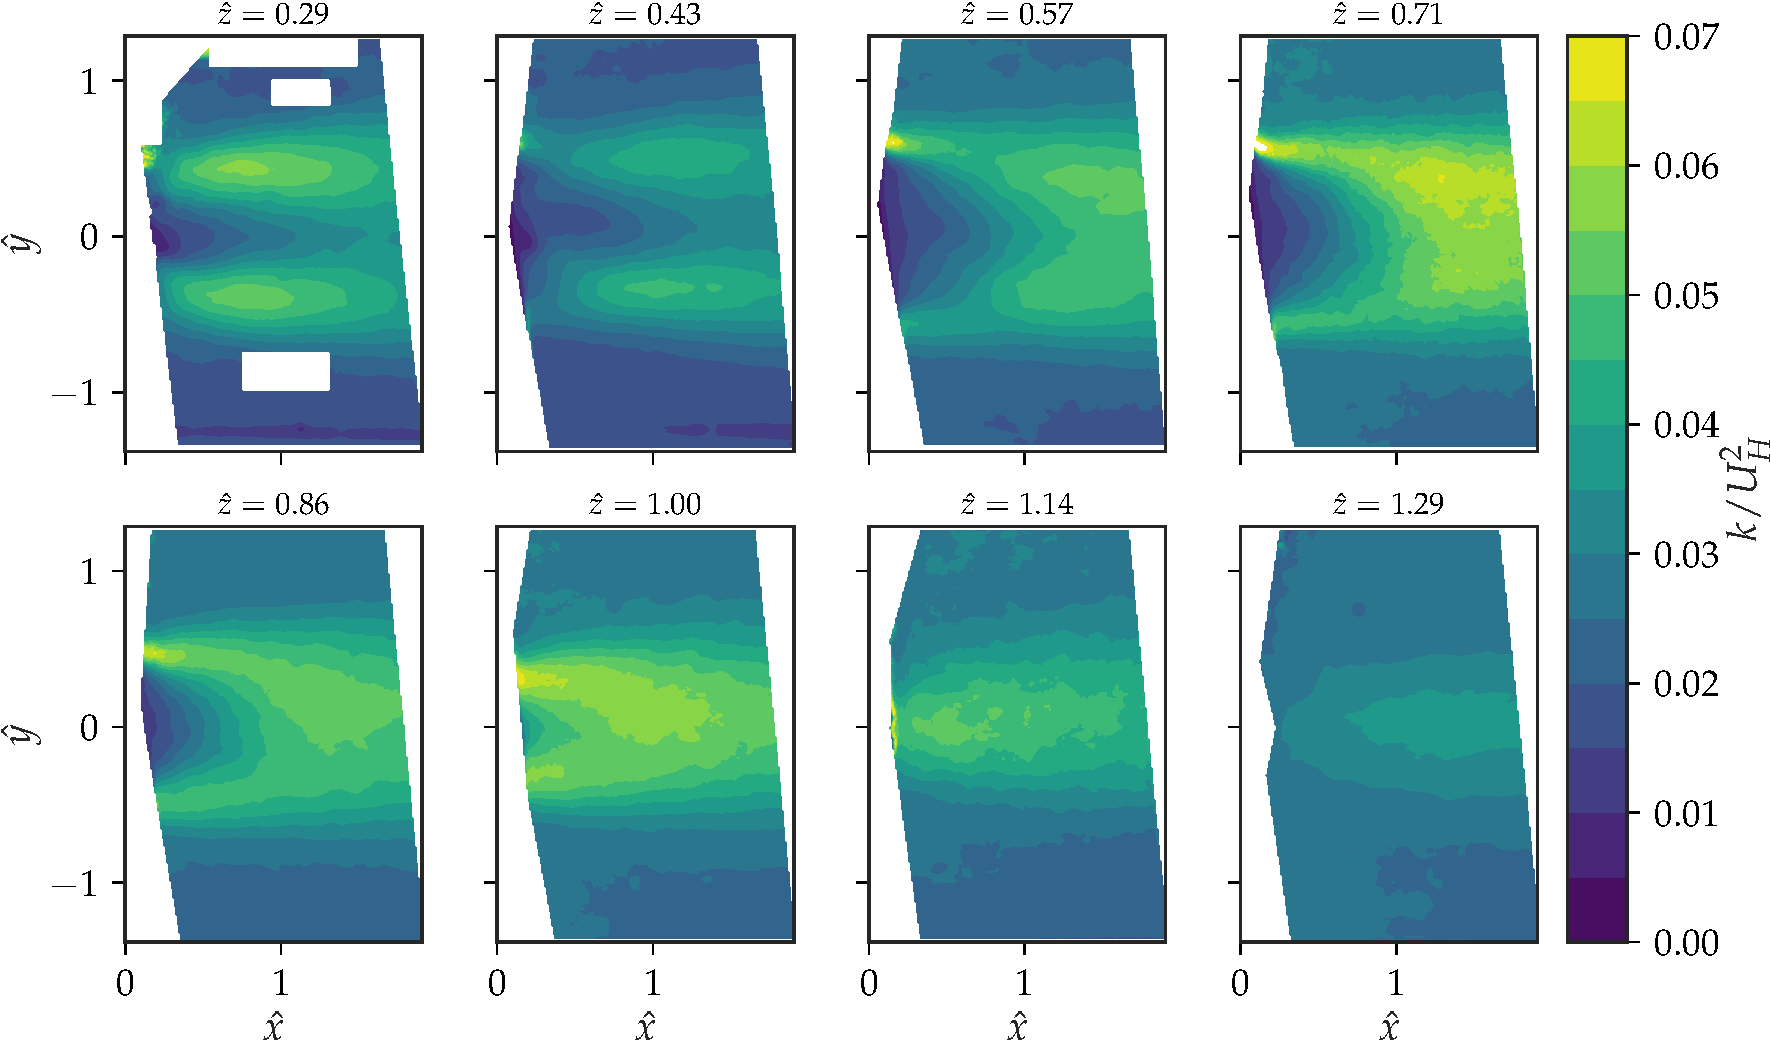
\includegraphics[width=\textwidth]{\figdir/hAll_TKE-crop.pdf}
		\caption{Normalized turbulent kinetic energy $k/U_H^2$ at 8 horizontal planes, $\hat{z}=$ [$0.29$,\,$0.43$,\,$0.57$, $0.71$, $0.86$, $1.0$, $1.14$, $1.29]$.}
		\label{fig:tke}
	\end{sidewaysfigure}


A more important impact of trees of the air flow is the turbulence modification resulted from the plant porosity. In literature, several studies emphasize the role of vegetation in turbulence enhancement for urban flows, which can drastically influence of the pollution dispersion and thermal characteristics \citep{Amorim2013,Gromke2008,Poggi2004}. The spatial variability in the turbulent kinetic energy (TKE) of the plant wake is investigated to understand the turbulence modification due to the porosity distribution. \cref{fig:tke} shows the normalized turbulent kinetic $k/U_H^2$ for the 8 horizontal planes. Trivially, the TKE is minimal in the freestream region and directly behind the plant (near  $\hat{x}= 0, \hat{y} = 0$ mm), where the flow is laminar or stagnated, respectively. In contrast, the TKE is high right near the shear zones at the transition between high and low wind speeds. Comparing different planes, we see that the TKE profile is high near the ground ($\hat{z}=0.29$) and near the plant canopy ($\hat{z}=1$). This again is attributed to the high shear flows generated from the boundaries of the plant foliage that is present at these two vertical levels. The exception to this a quantifiably high TKE regions for the vertical plane $\hat{z}=0.71$. Investigating, the vertical porosity of plant, \cref{fig:porosities}b, a dip in plant porosity is observed. Therefore, the increases in the TKE can result from the sudden variability in plant porosity, and we see the impact of porosity heterogeneity on the mixing characteristics.

\subsubsection*{Influence of porosity on wake turbulence}
	
	\begin{figure}[t]
		\centering
		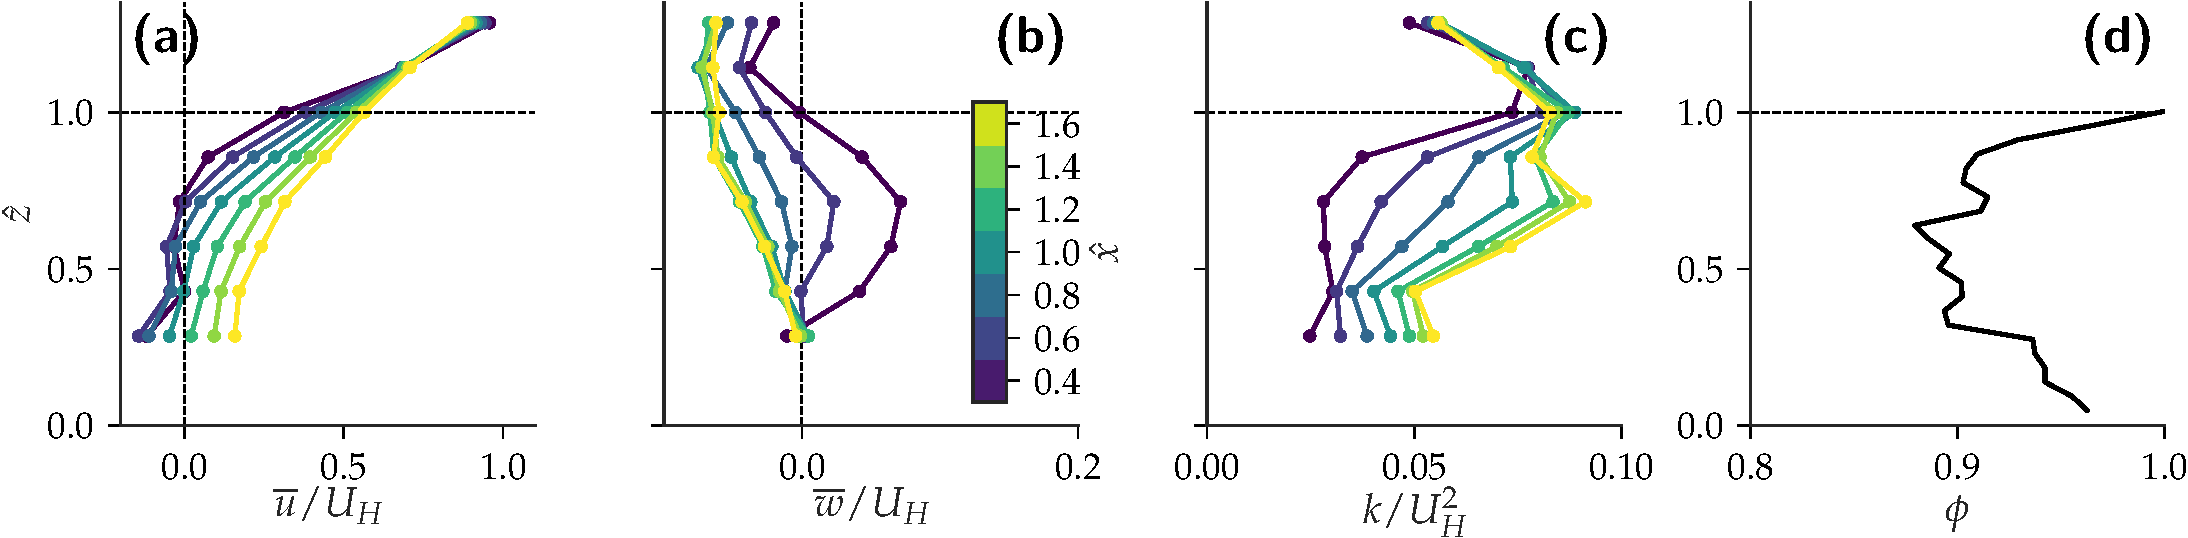
\includegraphics[width=\textwidth]{\figdir/figure_velocityprofile_centerline-crop.pdf}
		\caption{Mean vertical profiles at 7 streamwise positions $\hat{x}$ at center-line of the plant $\hat{y} = 0$: \subfig{a} streamwise velocity $\tavg{u}/U_H$ \subfig{b} vertical velocity $\tavg{w}/U_H$, \subfig{c}  turbulent kinetic energy $k/U_H^2$ and \subfig{d} streamwise-averaged porosity $\langle \phi \rangle_x$.}
		\label{fig:verticalprofile}
	\end{figure}

To better study the influence of plant porosity on the wake profile, the centerline flow statistics, and the plant porosity is compared in conjunction. \cref{fig:verticalprofile} shows the vertical profiles of the center-line velocity for 7 streamwise positions, $\hat{x} =$ $[0.4$, $0.6$, $0.8$, $1.0$, $1.2$, $1.4$, $1.6]$. At the vicinity of the trees and towards the lower half of the plant, the streamwise velocity $\tavg{u}$ is predominately negative. Furthermore, a positive vertical velocity $\tavg{w}$ is observed. This indicates a zone of strong circulation with reverse-flow configuration. Further downstream of the plant ($\hat{x}>0.8$), the streamwise velocity becomes positive and the vertical velocity becomes negative. Therefore, the flow characteristics is dominated by strong downwash of wind, bring high momentum velocity from above the plant canopy towards lower momentum regions of the ground. As such, the region is beyond the recirculation zone of the plant. The influence of porosity vertical variation on the mean velocities is not evident indicating no apparent correlation. However, the TKE profiles, especially away from the plant, shows a slight increase in TKE where the plant porosity is lower.

\subsection{Diurnal behavior of the plant}
\label{subsec:diurnal}

A thorough understanding of the plant morphology from section 3.1 and the resulting flow characteristics in \textbf{section 3.2} enables us now to obtain an understanding of the impact of the plant on the microclimate. The diurnal response of the plant and its daytime and nighttime averages are investigated. Thereafter, the dynamic characteristics during the transition between day and night are investigated. 

\subsubsection*{Influence of environment on diurnal response}

The diurnal behavior of the plant is investigated for two distinctly different boundary condition: no wind condition and wind condition with $U_{ref}=1$ m\,s$^{-1}$. \cref{fig:figure_transpirationrate} shows the diurnal variation of the water mass loss $m$ (g) throughout the day and night and the resulting the transpiration rate $TR$ (g\,h$^{-1}$), defined as:
\begin{equation}
TR = \frac{\mathrm{d}m}{\mathrm{d}t}
\end{equation}
measuring the hourly change in mass due to transpiration. We observe that during the night, regardless of the wind condition, a constant transpiration rate of $2.5$ g\,h$^{-1}$ exists. This transpiration rate, at the absence of solar radiation, is therefore associated to water loss simply due to respiration \citep{Farquhar1980, Lambers2008, Launiainen2015}. At dawn, a stark increase in transpiration rate is observable. Furthermore, at this time, the wind condition plays an important role as during wind condition, a peak transpiration rate of $15$ g\,h$^{-1}$ is observed. Whereas, without wind, the transpiration rate peaks only at $10$ g\,h$^{-1}$. This dynamic response results from the delay in stomatal response. A detailed investigation of this hysteresis is presented in \cref{subsec:dynamic}. As the day progresses, the stomatal regulation is seen to compensate the influence of wind, resulting in similar transpiration rate with an average transpiration rate of $9$ g\,h$^{-1}$. However, by the course of the day, the transpiration is seen to decay quantifiably. Such decay in the daytime transpiration rate has also been observed previously \citep{Javaux2013, Tuzet2003}. The phenomenon is attributed to the reducing rhizosphere soil moisture. The reduced soil moisture eventually reduces the stomatal conductance, resulting in the decayed transpiration rate that we observe. However, at night, the soil moisture equilibrates as the root water uptake is drastically diminished to only $2.5$ g\,h$^{-1}$. 

	\begin{figure}[t]
	\centering
	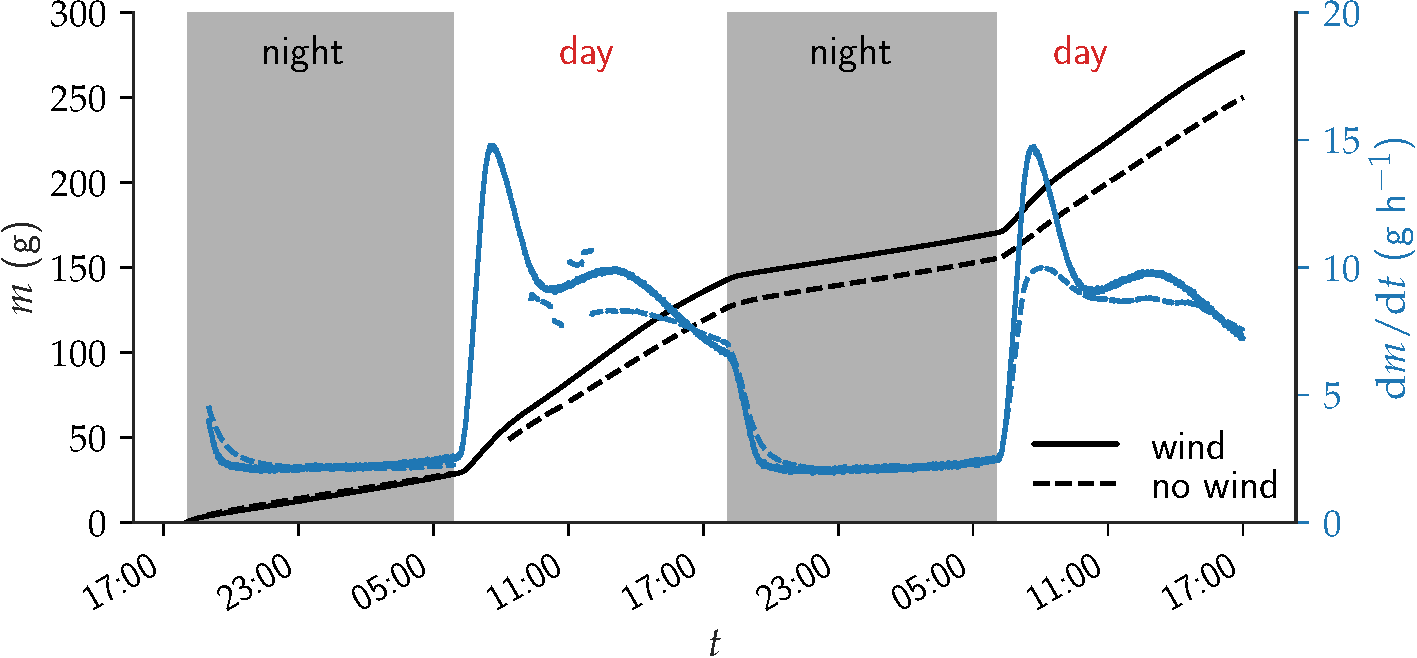
\includegraphics[width=\textwidth]{\figdir/figure_transpirationrate-crop.pdf}
	\caption{Diurnal variation of mass loss $m$ (g) and the resulting transpiration rate $TR=\mathrm{d}m/\mathrm{d}t$ (g h$^{-1}$) for two wind conditions: \textit{no wind} and \textit{with wind} ($U_{ref}=1$ m\,s$^{-1}$).}
	\label{fig:figure_transpirationrate}
	\end{figure}

The influence of the varying transpiration rate is further investigated by studying the microclimate variables, air temperature T ($^{\circ}$C) and relative humidity RH (\%) inside the plant foliage. The setup of the microclimate sensors is detailed in \cref{subsec:windtunnelsetup}. \cref{fig:figure_airtemperature_humidity_v2} shows the diurnal variation of the air temperature and relative humidity inside the tree at various heights, with $T_1$ at the bottom of foliage and $T_6$ at the plant canopy ($H=210$ mm). The configuration is such that probes 1 to 5 are directly inside the plant foliage with $30$ mm offset. Furthermore, the ambient condition (``\textit{air}'') and the ground condition below the plant (``\textit{ground}'') is compared to study the influence of plant shading. \textbf{Fig. 14} shows that in the no wind condition, there is a quantifiable drop in the air temperature and a substantial increase in the relative humidity, with peak $RH=75$\% during day time. During the night, vertical variability in a microclimate within the foliage is smaller but still noticeable. All the sensors inside the plant foliage shows an improved thermal condition with lower temperature during day and night. However, the sensor at plant canopy ($H=210$ mm), shows that air temperature is noticeable higher than the ambient condition. This indicates that the plant canopy region is strongly influence by the absorption of solar radiation, leading to higher leaf temperature and positive sensible heat flux, thereby heating up the air. Similar observation of positive sensible heat flux due to high solar radiation absorption have also been observed numerically \citep{Manickathan2018a}. However, in the shadow of the plant, we see that air temperature is lower than sunlight region. This could be attributed to the secondary cooling (i.e., the cooling due to the ground) as the shaded ground has less thermal energy. 

	\begin{figure}[t]
	\centering
	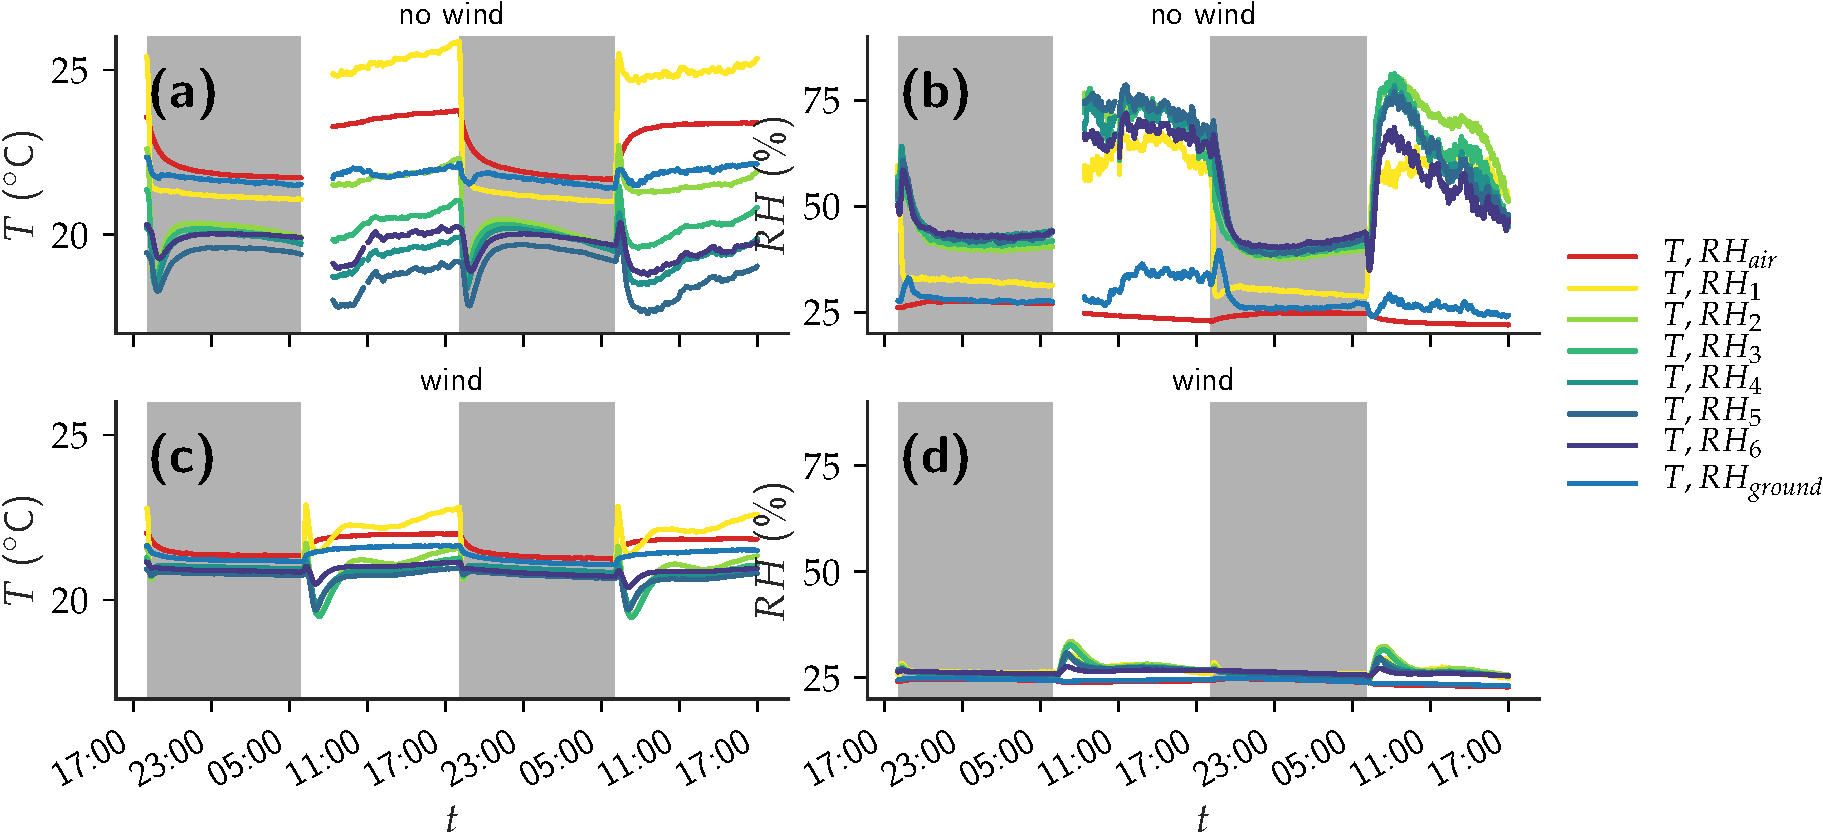
\includegraphics[width=\textwidth]{\figdir/figure_airtemperature_humidity_v2-crop.pdf}
	\caption{Diurnal variation of air temperature $T$ ($^{\circ}$C) and relative humidity $RH$ (\%) inside the tree at varying heights for two wind conditions: \subfig{a}\subfig{b} \textit{no wind} and \subfig{c}\subfig{d} \textit{wind} ($U_{ref}=1$ m\,s$^{-1}$).}
	\label{fig:figure_airtemperature_humidity_v2}
	\end{figure}

The impact of transpiration of the microclimate is quickly diminished at the presence of wind. The wind conditions reduced the benefit of transpirative cooling due to increased ventilation of the plant foliage. Therefore, the maximum humidity within the plant is similar to ambient condition outside the plant. The influence of wind on transpiration rate is complex as we observed in \cref{fig:figure_transpirationrate}, the relative humidity inside the plant changes, the leaf temperature changes, and so, the vapor pressure gradient will also be different \citep{Manickathan2018a}. Furthermore, stomatal resistance is also a function of the VPD and so in our case transpiration rate is also affected. At dawn, we observe a large transpiration rate, however, by midday, equalizes to no wind condition. The observation is contrary to what is typically mentioned in literature, where the Penman-Monteith equation predicts a decrease in transpiration rate due to wind speed \citep{Dixon1983, Schymanski2016}. However, it is also mentioned that the type of species also has an influence \citep{Dixon1983}. 

\subsubsection*{Comparison of day and night plant response}

The average daily response of the plant and its influence on the climate is studied to understand the influence of vegetation. \cref{fig:figure_airtemperature_relativehumidity_profile} shows the median air temperature at various height for the case with wind and without wind, respectively. The figure furthermore differentiates the daytime and nighttime median air temperature. The figure shows, trivially, that the air temperature change is largest during the day. However, more interesting, the figure shows that during the wind case, the air temperature inside the tree is more homogenized, whereas, during the case of no wind, a large vertical variability is observable. Hence, we investigate the vertical heterogeneity in the air temperature and the relative humidity. We see that the most significant cooling, i.e., providing the largest drop in air temperature, is present for the no wind condition during the day for heights between $0.29\le\hat{x}\le0.57$. During this condition, we also observe a large increase in the relative humidity. During wind condition, and especially at night, the vertical variability in relative humidity and air temperature is diminished. This indicates that the cooling is only prevalent when transpiration is high and when the air is stagnated inside the plant, such that transpiration-driven cooling can effectively extract the thermal energy of the stagnated air. When, we investigate the influence of vertical porosity variation, we see no evident correlation on the thermal or moisture distribution. The key driving factor is the solar radiation intensity, which is highest at the plant canopy, and quickly decays into the foliage \citep{Manickathan2018a}. Such gradient in radiation absorption, results in the observed air temperature spike at plant canopy as indicated by sensor 6. The probes 1 to 5 that are within the foliage, which are protected from the solar radiation, shows a significantly lower air temperature.

	\begin{figure}[t]
	\centering
	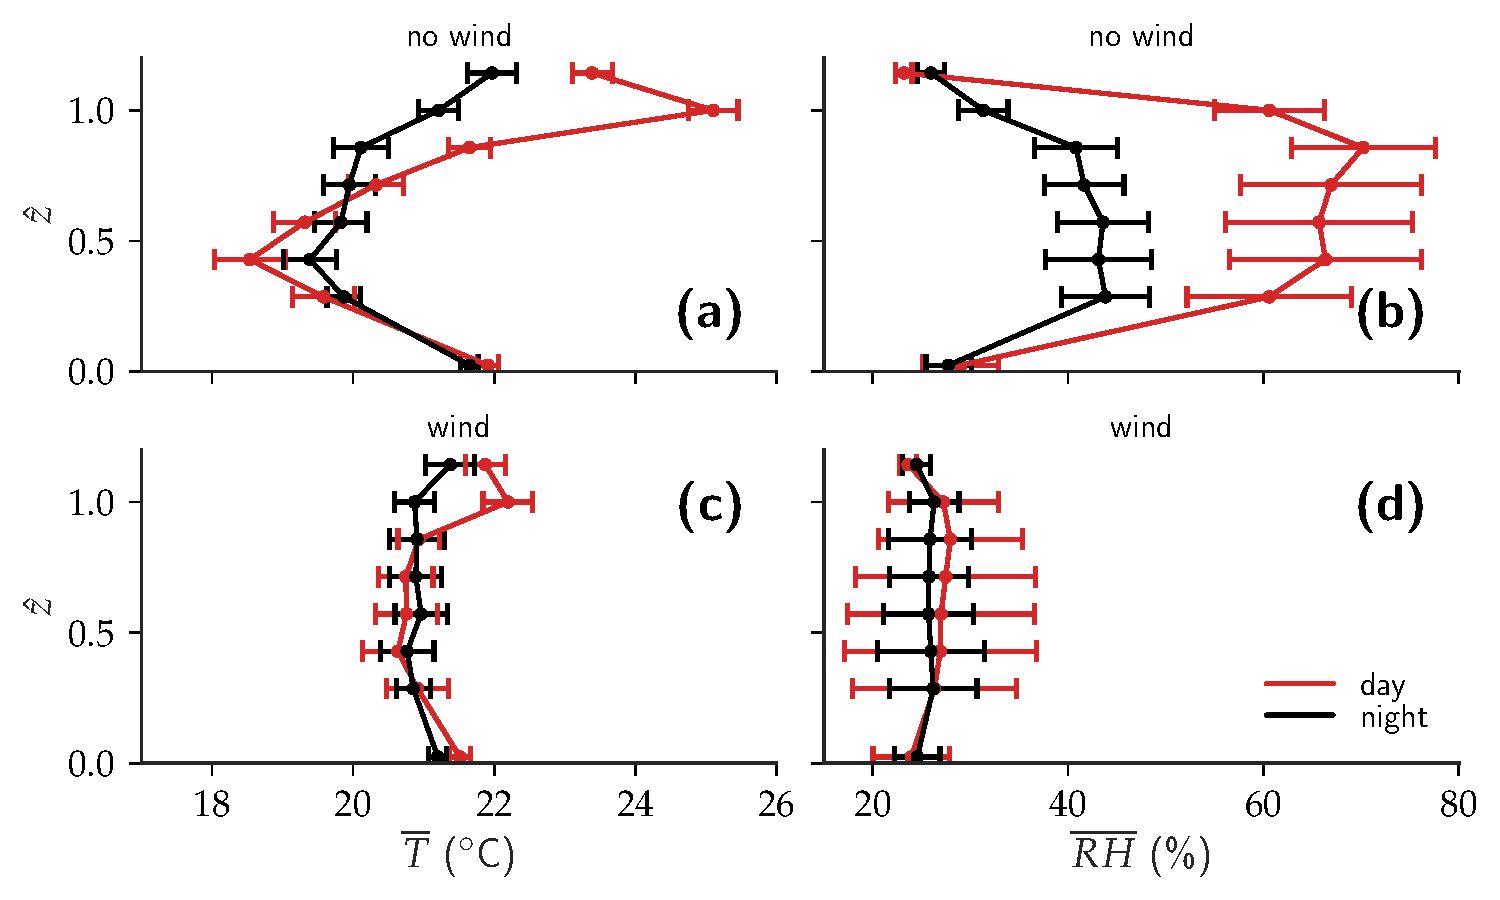
\includegraphics[width=\textwidth]{\figdir/figure_airtemperature_relativehumidity_profile.pdf}
	\caption{Mean vertical distribution of day (red) and night (black) \subfig{a}\subfig{c} air temperature $T$ ($^{\circ}$C) and \subfig{b}\subfig{d} relative humidity $RH$ (\%) inside the tree for two wind conditions: \subfig{a}\subfig{b} \textit{no wind} and \subfig{c}\subfig{d} with \textit{wind} ($U_{ref}=1$ m\,s$^{-1}$).}
	\label{fig:figure_airtemperature_relativehumidity_profile}
	\end{figure}


To investigate the influence of transpiration on leaf temperature, the leaf temperature is measured through infrared thermography. \cref{fig:IR_dayvsnight_windvsnowind_type2_v2} shows the diurnal variation of leaf surface temperature for wind and no wind condition. The thermography shows that during the wind condition, the spatial variability in leaf temperature is minimal, especially during the night. Therefore, the convective exchanges equilibrate the leaf temperature variability arising from solar radiation. This is especially evident when observing the no wind condition. During the no wind condition, the vertical heterogeneity in leaf temperature is clear showing higher plant canopy leaf temperature and a cooler in foliage leaf temperature, especially at the lower regions. \cref{fig:IR_dayvsnight_windvsnowind_type2_v2}c and \cref{fig:IR_dayvsnight_windvsnowind_type2_v2}d shows the difference between the wind and no wind condition for night and day, respectively. During the night, the difference between no wind and wind condition is minimal with wind condition leaf temperature being slightly higher. Near the plant canopy, the leaf temperature difference for ``\textit{with wind}'' condition is substantially higher, indicating that when the wind is present, the leaf temperature is lower through the increased convective heat flux. The impact of higher leaf temperature is also reflected as previously observed in the air temperature,\textbf{ Fig. 15}. Moreover, the enhanced cooling observed during no wind condition during the day (\textbf{Fig. 15a}), is also reflected by the lower leaf temperature shown in \cref{fig:IR_dayvsnight_windvsnowind_type2_v2}d.

	\begin{figure}[t]
	\centering
	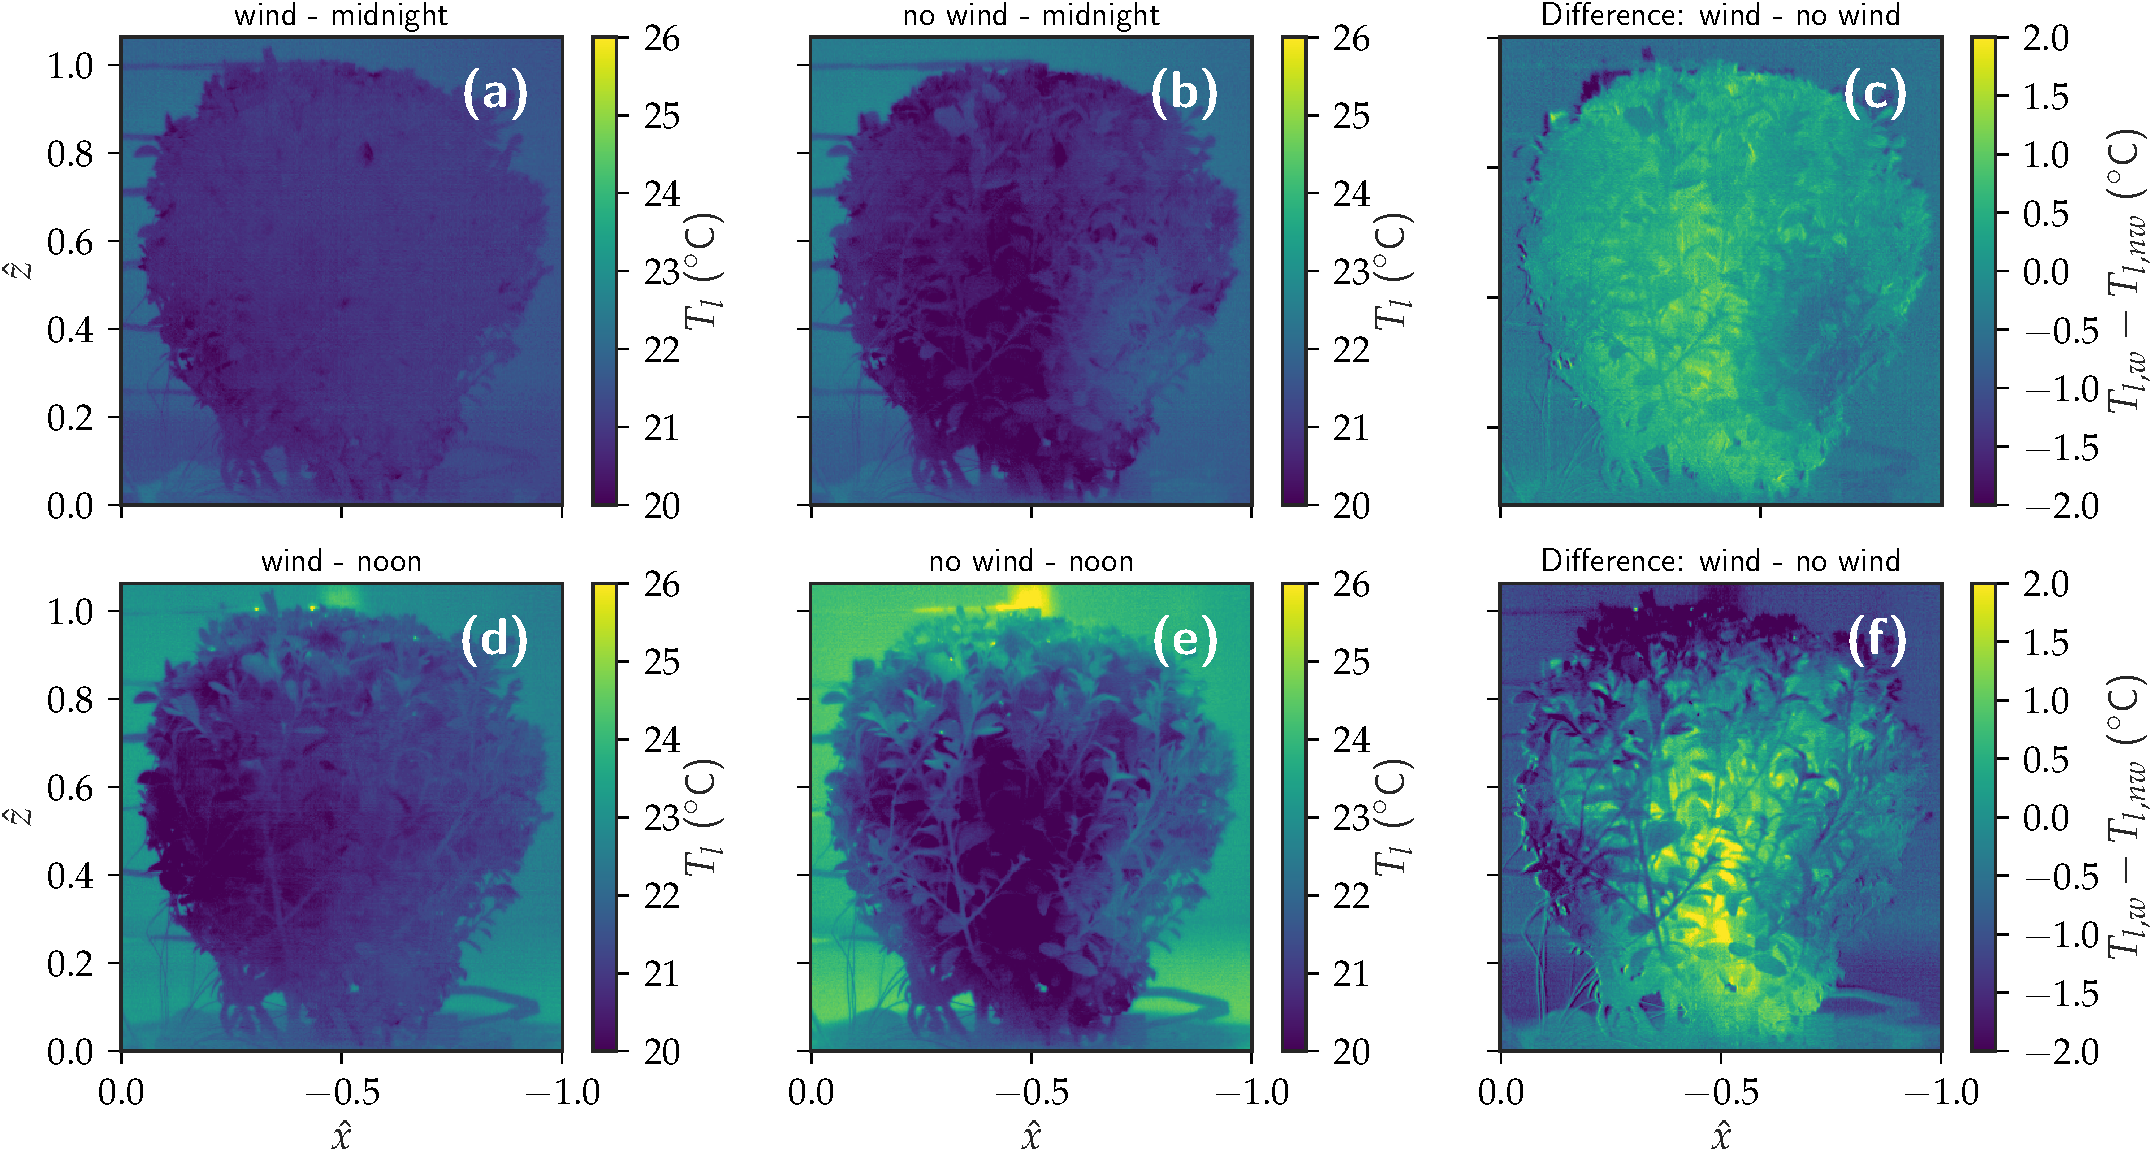
\includegraphics[width=\textwidth]{\figdir/IR_dayvsnight_windvsnowind_type2_v2-crop.pdf}
	\caption{Diurnal variation of leaf surface temperature $T_l$ ($^{\circ}$C) at \subfig{a}\subfig{b}\subfig{c} nighttime (midnight) (\subfig{d}\subfig{e}\subfig{f}  and midday (noon). The difference between \textit{wind} and \textit{no wind} condition is compared for \subfig{c} night and \subfig{f} day.}
	\label{fig:IR_dayvsnight_windvsnowind_type2_v2}
	\end{figure}


\subsection{Dynamic response of the plant}
\label{subsec:dynamic}

During the transition between day and night, a smaller time scale dynamic is observed, influenced by the abrupt changing in the environmental condition. \cref{fig:IRimage_phasediagram_type3} shows the spatiotemporal variability of streamwise-averaged leaf temperature $\langle T_l \rangle_x $ for \textit{no wind} and \textit{wind} condition. The figure shows the vertical variability in leaf temperature over the progression of the day. We see that, as observed with the internal microclimate of the plant (\cref{fig:figure_airtemperature_relativehumidity_profile}), the variability is only prevalent during the day time. Furthermore, the no wind condition shows stronger variability than the wind condition. During the day at no wind condition, a temperature spread from $19$ to $25$ $^{\circ}$C is observed. Moreover, we see that the leaf temperature is not only dependent on the vertical height, but also the time of the day. At the initial moments of dawn, the leaf temperatures quickly rise with highest temperatures observed at the plant canopy, showing a high gradient in leaf temperature where the leaves are exposed to solar radiation. We see that thereafter, the stomatal regulatory function takes over and a drastic decrease in foliage temperature is observable, especially in the middle regions of the foliage with  $T_l \approx 19$ $^{\circ}$C. As the day progress however, the cooling effect diminishes, and the foliage temperature starts to rise again. Just before dusk, a plant foliage temperature is similar to the onset of dawn, with high plant canopy temperatures. 

	\begin{figure}[t]
	\centering
	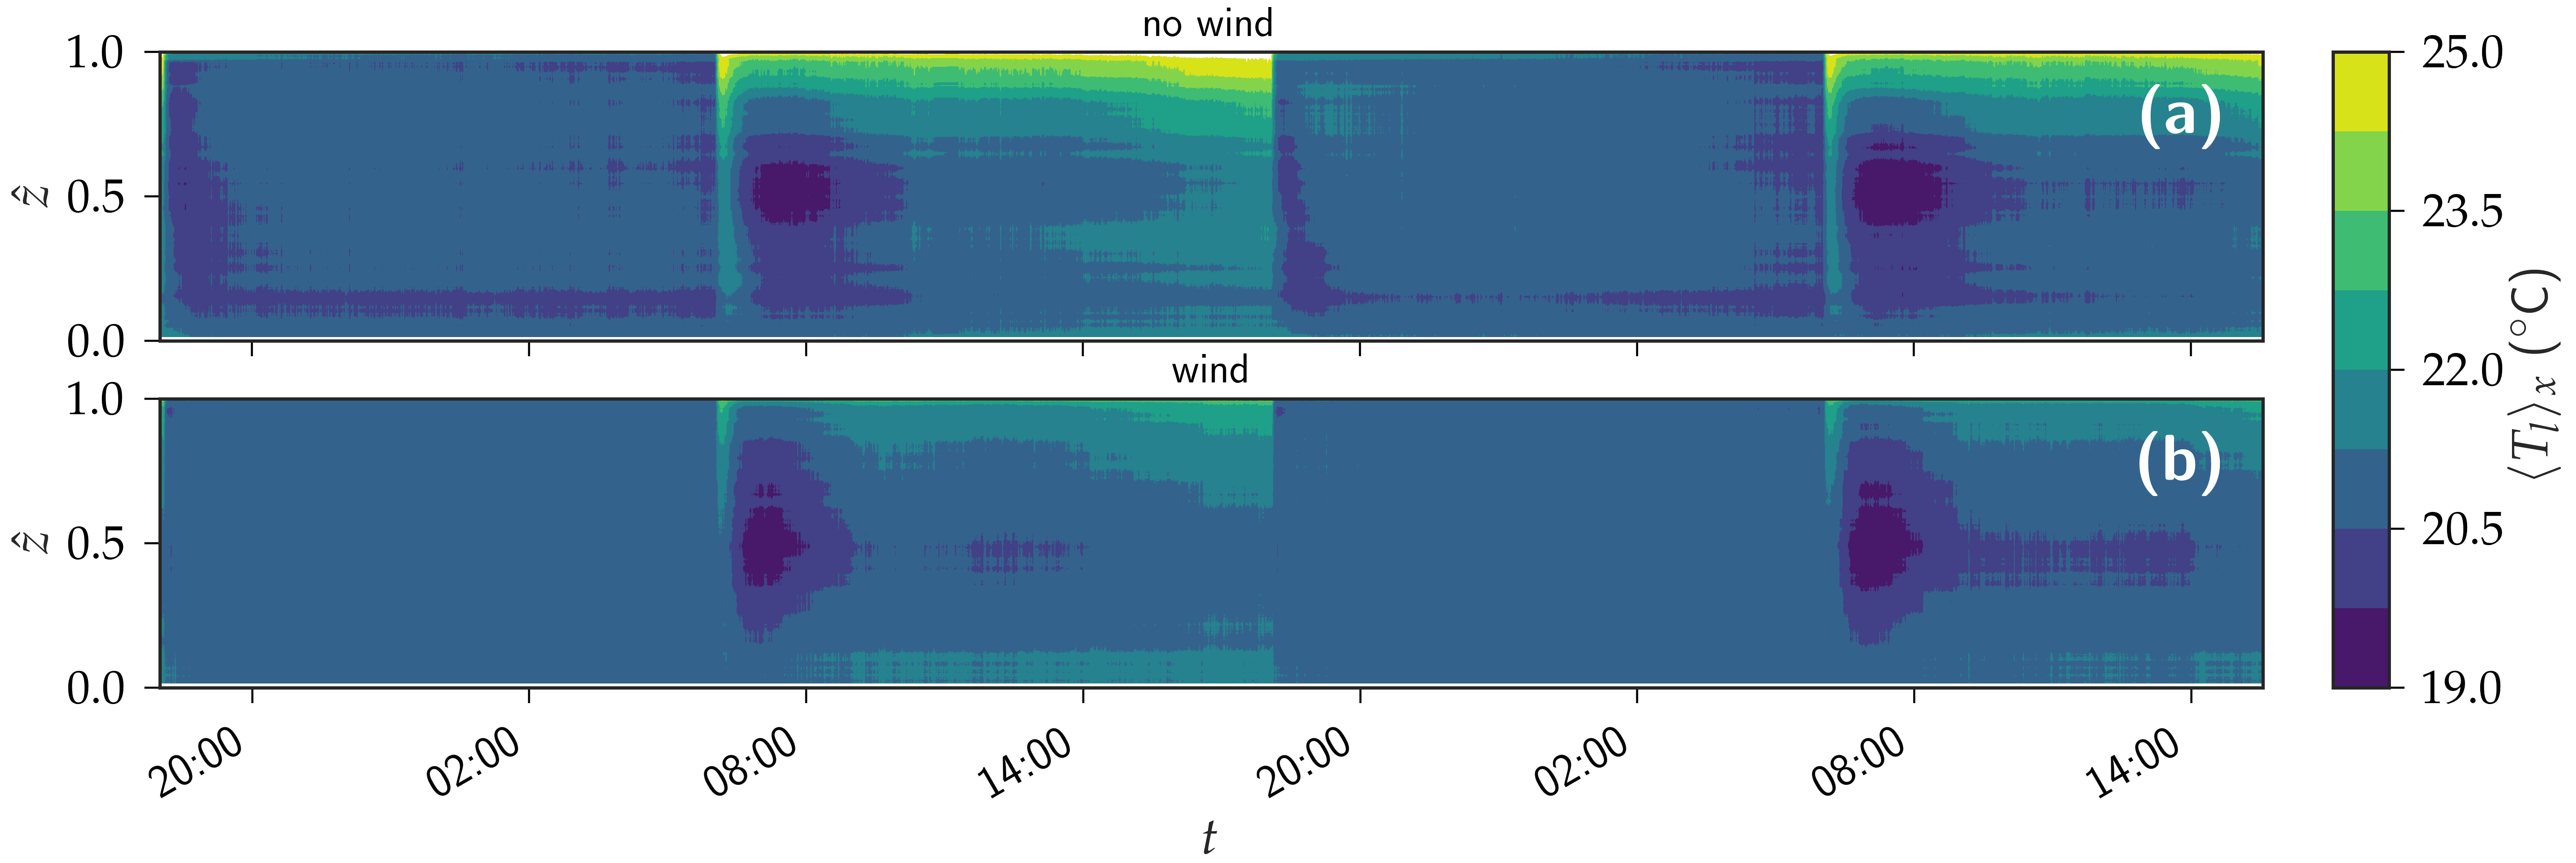
\includegraphics[width=\textwidth]{\figdir/IRimage_phasediagram_type3.png}
	\caption{Streamwise-averaged spatiotemporal variability of leaf temperature $\langle T_l \rangle_x$ ($^{\circ}$C) comparing \subfig{a} \textit{no wind} and \subfig{b} \textit{wind} condition.}
	\label{fig:IRimage_phasediagram_type3}
	\end{figure}

\cref{fig:Tprofile_2} shows the diurnal progress of the net spatial-averaged leaf temperature $\langle T_l \rangle_{xz}$ comparing wind and no wind condition. We notice that the no wind condition simply amplifies the characteristics that is present during the wind condition. Furthermore, we see that the day is composed of four unique stages: overshoot, overcorrection, equilibration and decay periods. The overshoot period is present at the initial stages of dawn where the leaves absorb solar radiation and stomata response has not been prevalent to provide the adequate transpiration rate. The delayed response of the plant results in the high overshoot of leaf temperature, which is compensated and corrected by the plant thereafter. However, we see that during the overcorrection period, the transpiration rate spikes, as evident from plant transpiration rate measurement, \cref{fig:figure_transpirationrate}, resulting in the drastic cooling measured. By midday, the stomatal response equilibrates the necessary transpiration rate and we observe a quasi-steady leaf temperature and transpiration rate (\cref{fig:figure_transpirationrate}) and in-foliage air temperature (\cref{fig:figure_airtemperature_humidity_v2}). Furthermore, it is shows that the equilibrium leaf temperature of plant foliage during no wind condition is higher than the wind condition. This is the result of the overall higher plant canopy temperature due to the reduces convective heat transfers. As the day progress, the leaf temperature transitions to the fourth stage with a slow increase in the leaf temperature. The observation correlates with the measured plant transpiration rate, \cref{fig:figure_transpirationrate}, where an equally decaying transpiration rate is observable. 

	\begin{figure}[t]
	\centering
	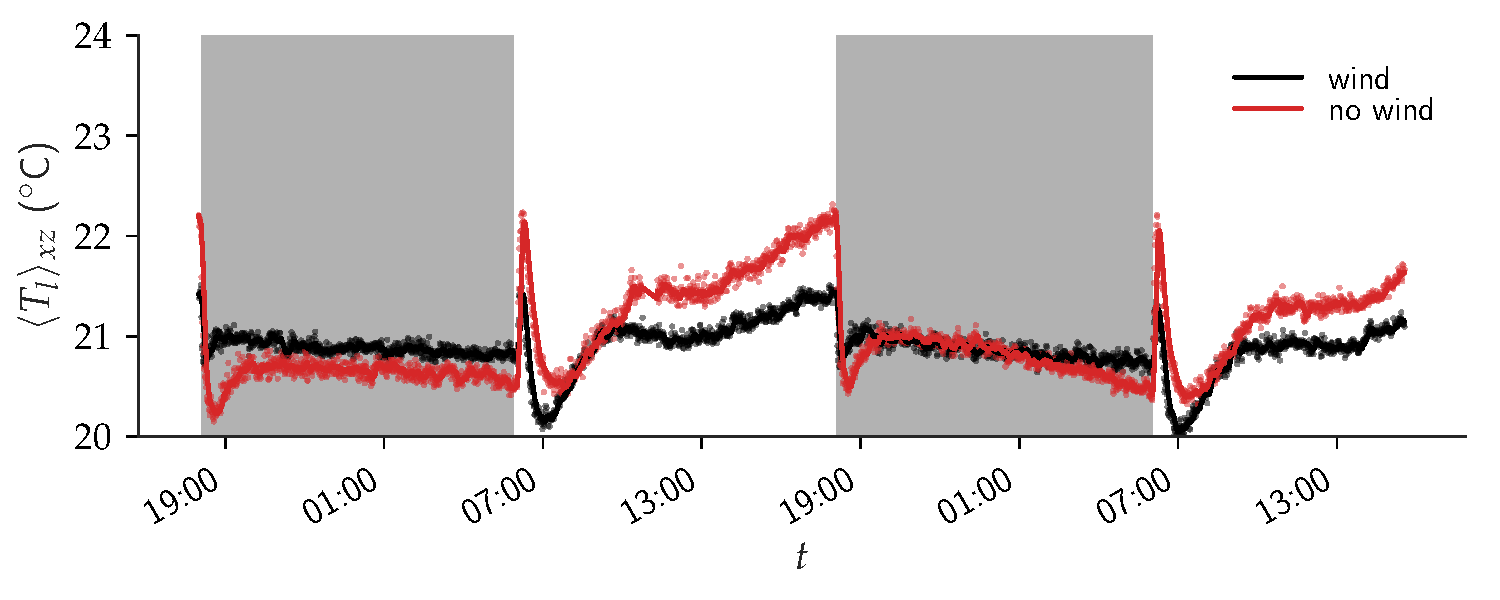
\includegraphics[width=\textwidth]{\figdir/Tprofile_2.pdf}
	\caption{Diurnal variation of spatially-averaged leaf temperature $\langle T_l \rangle$ ($^{\circ}$C) for \textit{wind} and \textit{no-wind} conditions.}
	\label{fig:Tprofile_2}
	\end{figure}

	\begin{figure}[t]
	\centering
	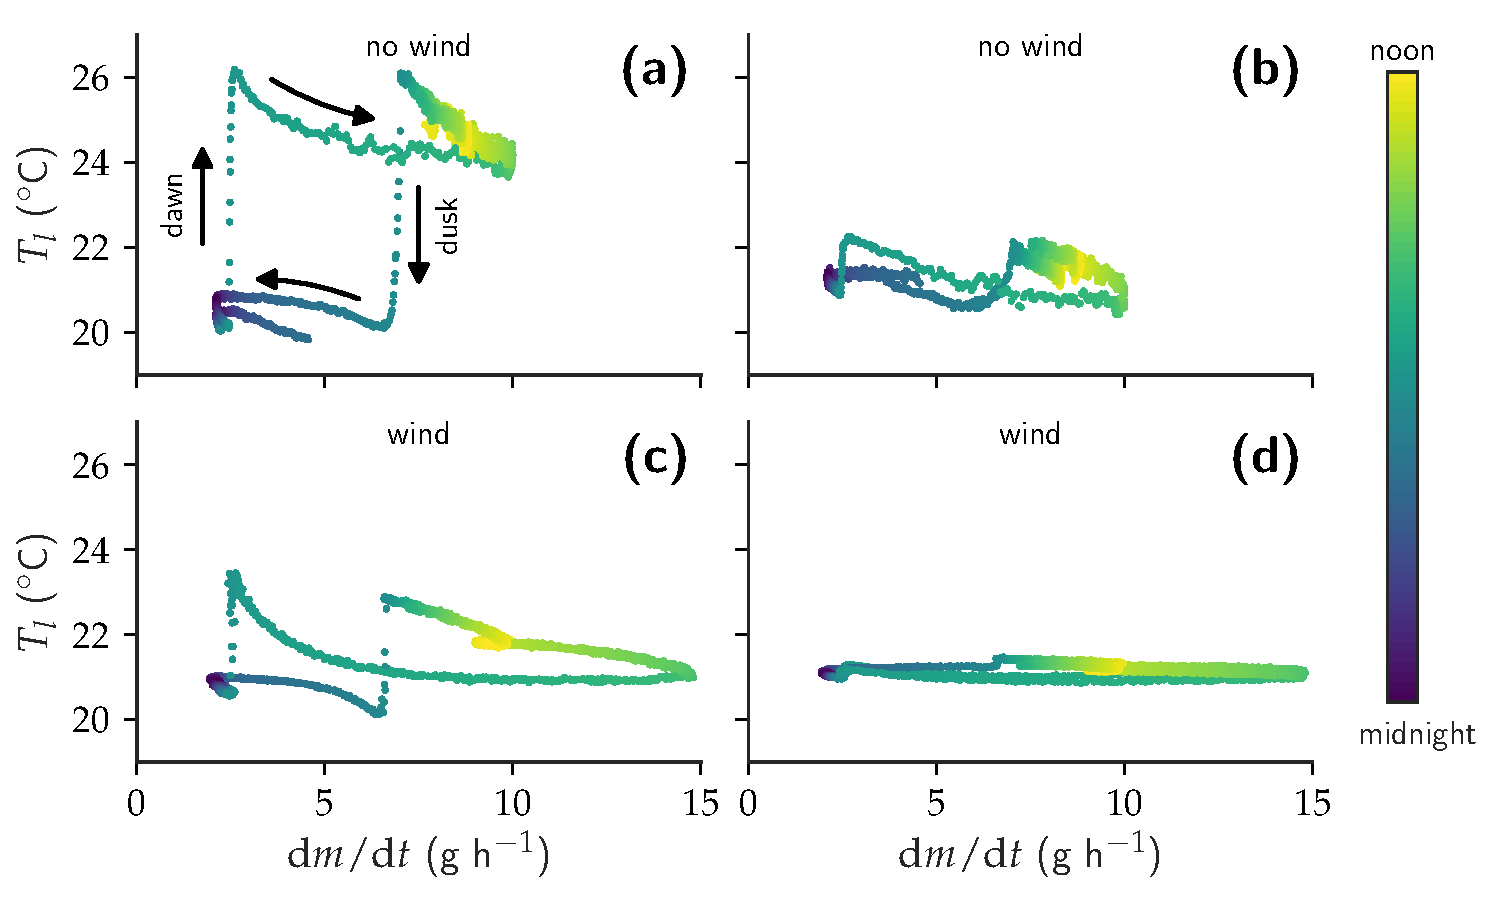
\includegraphics[width=\textwidth]{\figdir/hysteresis_transpirationrate_vs_temp_v2.pdf}
	\caption{Diurnal variation of $TR=\mathrm{d}m/\mathrm{d}t$ (g\,h$^{-1}$) and leaf temperature for two wind conditions: \subfig{a}\subfig{b}  \textit{no-wind} and \subfig{c}\subfig{d}  with \textit{wind} ($U_{ref}=1$ m\,s$^{-1}$). The leaf temperatures are obtained from \subfig{a}\subfig{c} plant canopy region and \subfig{b}\subfig{d}  near the ground region of the foliage.}
	\label{fig:hysteresis_transpirationrate_vs_temp_v2}
	\end{figure}

\cref{fig:hysteresis_transpirationrate_vs_temp_v2} shows a clearer hysteresis between net the leaf temperature and the net plant transpiration rate. The leaf temperatures of sunlight foliage and sunshade foliage are compared with the net plant transpiration. In all cases, a cyclic pattern of leaf temperature and transpiration rate is observable. Furthermore, we see that the hysteresis is amplified for the sunlight region during the no wind condition. At dawn, we see the overshoot as observed in \cref{fig:Tprofile_2}. After a delay, the stomata respond to the solar radiation and provide the necessary transpiration rate to cool the leaves. \cref{fig:IRimage_phasediagram_type3} shows this delayed cooling of the leaves observed through infrared thermography and the subsequent cooling of the air temperature, \cref{fig:figure_airtemperature_humidity_v2}, measured from the SHT sensors. However, towards dusk, we observe that the leaf temperatures slowly start to rice. An equivalent reduction in the plant transpiration rate is also observable from the hysteresis diagram, \cref{fig:hysteresis_transpirationrate_vs_temp_v2}. At the end of the photo-period, we observe a sudden drop in the leaf temperature. However, the plant transpiration rate is seen not to respond at the same rate as the decay in observed leaf temperature. Only after the leaf temperature equilibrated to a lower level is the stomata seen to respond, as indicated by the change in transpiration rate. The result is a cyclic nature of the plant transpiration rate, and the leaf temperature resulted from the delayed response of the plant. A similar observation of hysteresis between plant transpiration and the root water uptake has been known in the literature \citep{Dauzat2001, Williams1996}. An essential aspect of this hysteresis is that such dynamic response of the plant is difficult to parameterize in urban climate models of vegetation. Only after an explicit modeling on the water transport within the plant can such phenomena be captured \citep{Huang2017, Manzoni2011}.



\section{Conclusion}

The goal of the present study was to unveil the diurnal changes in plant microclimate using multiple non-intrusive imaging techniques such as stereoscopic particle image velocimetry (SPIV) for the flow field, infrared thermography for the leaf temperature and X-ray tomography for the plant microstructure. The present study aimed at answering the following questions: What are the spatial and temporal variability of the plant performance due to environmental conditions such as wind speed and solar radiation? What is the diurnal response of the plant? 

The high-resolution measurement of the plant porosity through X-ray tomography enabled us to find that that the aerodynamic and optical porosity typically used in the wind tunnel studies does not reflect the true porosity distribution of the plant. Moreover, the paper presents a novel approach of determining the leaf area density a directly from X-ray tomography. The advantage of this non-intrusive approach of determining the plant microstructure enabled us to fit series of additional experiments, enabling us to directly quantify the impact of plant foliage morphology on the wake flow characteristics, the hygrothermal conditions such as air temperature and relative humidity inside the plant foliage, the solar radiation penetration inside the foliage and, finally, its impact on the spatial distribution of the leaf temperature. The SPIV measurement of the wake flow field helped us to find that at regions where porosity $\phi\rightarrow 1$, a strong bleed flow is observable, indicated by the mean velocity component. However, in contrast, there was no apparent link between the plant porosity distribution and the turbulent kinetic energy (TKE). The TKE intensity was seen to be governed by the net plant porosity and the outer geometry of the plant foliage that generates the shear-layer and how it interacts with the upstream boundary layer profile.

The hygrothermal measurement at multiple vertical locations within the plant foliage enabled us to find that the local cool ``\textbf{oasis}'' generated by transpirative cooling, quickly diminished when the wind is present. The diurnal measurement of the transpiration rate showed that the water use efficiency (WUE) changes during the day indicated by the decaying transpiration rate. Furthermore, the high-resolution infrared thermography measuring the spatial and temporal changes in the leaf temperature revealed further dynamic variability during the day. A comparison of the diurnal variation in the leaf temperature and the net plant transpiration rate enabled us to quantify the diurnal hysteresis resulting from the stomatal response lag. The day is seen to comprise of four unique stages: \textit{no-cooling} (i.e., the stage when stomata has not responded to the increase in solar radiation), \textit{high-cooling} (i.e., when stomatal response tries to compensate for increased leaf temperature), \textit{equilibrium} (i.e., when stomatal response and leaf temperature equilibrates) and \textit{decaying-cooling} stage (i.e., when the transpiration rate starts to weaken). Such plant responses are difficult to parameterize and simplify for urban climate-vegetation models without explicitly modeling the water transport within the plant. The downside is that simplified models might not be able to predict rapid changes in leaf temperature due to the sudden change in atmospheric evaporative demand (AED) resulting from sudden change in solar radiation (e.g. due to sudden change in cloud cover) or sudden change in wind speed (ex. due to gust). Therefore, higher-fidelity models of plant responses should take such dynamics that arise from water availability and the stomatal response delay, to accurately assess the transpirative cooling potential of vegetation. The outlook of the present paper is to provide high-resolution multivariate measurement dataset for development and validation towards such advanced numerical methods. 



%\begin{figure}[t]
%\centering
%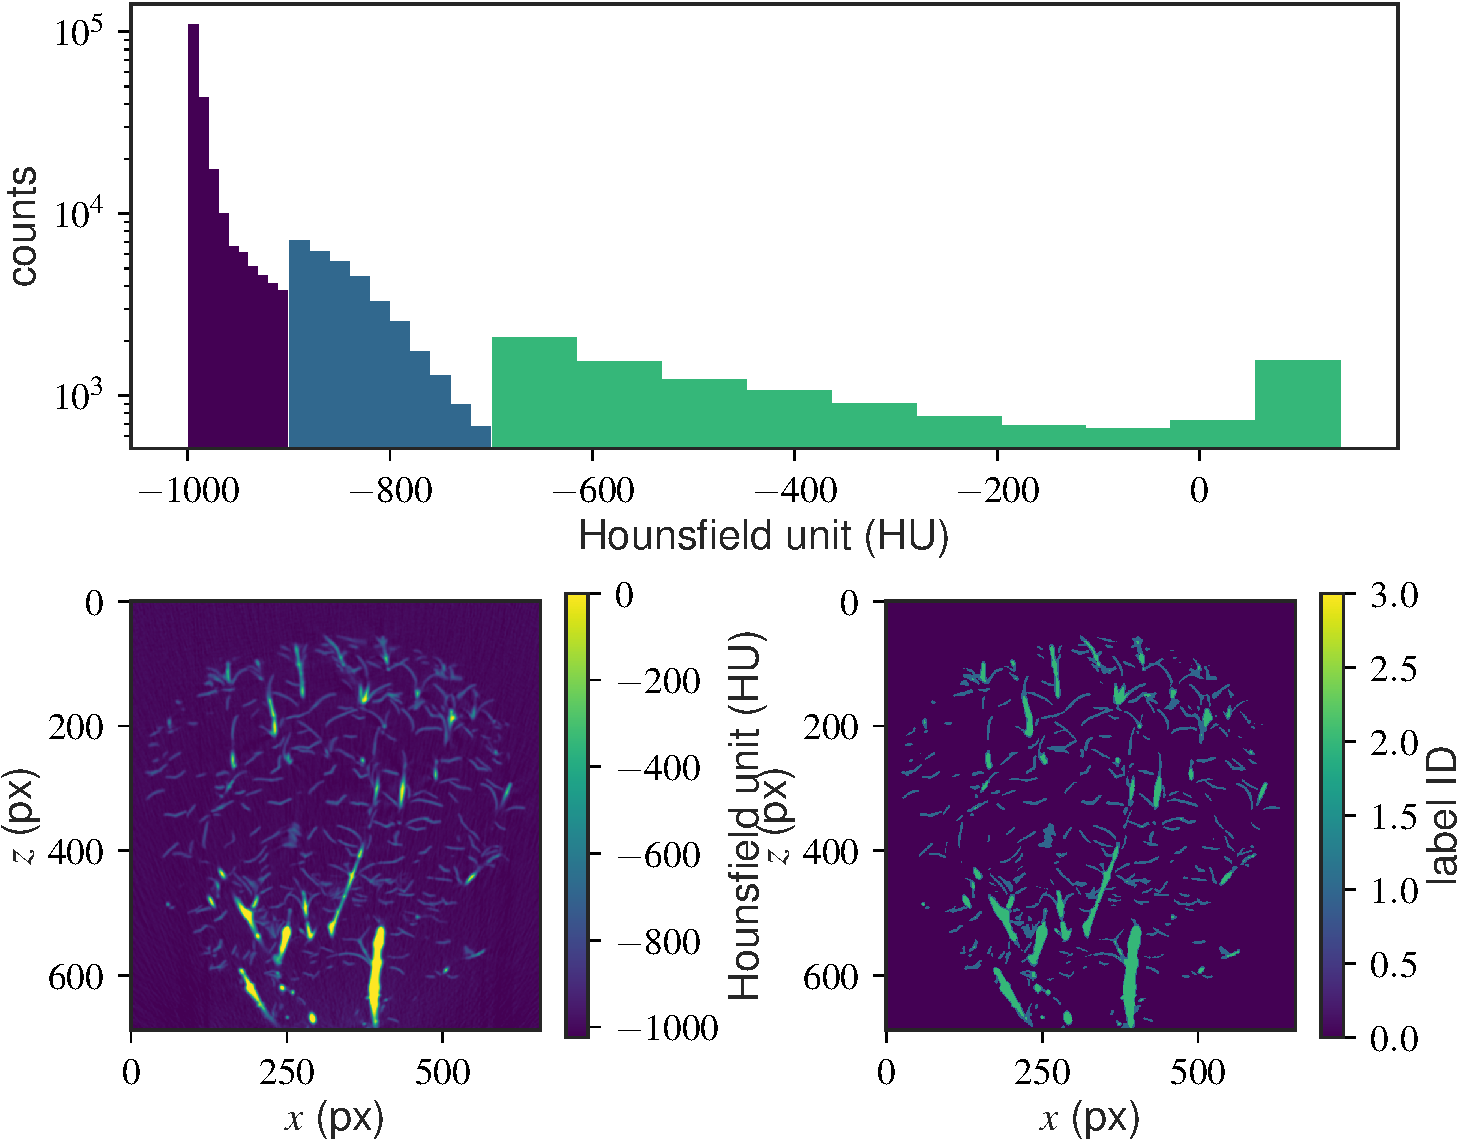
\includegraphics[width=\textwidth]{\figdir/figure_histogramsegentation-crop.pdf}
%\caption{Segmentation of the x-ray CT scan: a) original x-ray CT data, b) segmentation using user-defined histogram thresholding and c) segmentation using trainable WEKA segmentation and additional morphological operation (opening and closing). A sub-region of an image slice is shown for clarity.}
%\label{fig:figure_histogramsegentation}
%\end{figure}